\documentclass[12pt]{article}                               % Make it an article
\usepackage{indentfirst}                                    % All subsections indented
\usepackage{setspace}                                       % For 1.5 spacing
\usepackage{hyperref}                                       % Make table of contents clickable, allow URLs
\usepackage[letterpaper, margin=1in]{geometry}              % 1 inch margin, letter paper (American)
\usepackage[english]{babel}                                 % For "fancy" quotes
\usepackage[autostyle, english=american]{csquotes}          % Same
\usepackage{apacite}                                        % Use APA citations
\usepackage{etoolbox}                                       % Misc
\usepackage{titlesec}                                       % Modify spacing
\usepackage{listofauthorships}                              % CUSTOM BUILT (lifted & edited from S/O)! Adds a table of authorship
\MakeOuterQuote{"}                                          % For fancy quotes
\usepackage{times}                                          % For tilde
\usepackage{textcomp}                                       % For tilde
\usepackage{graphicx}                                       % Images
\usepackage{array}                                          % Table spacing
\usepackage{ragged2e}                                       % Left align table text
\usepackage{caption}                                        % Use to create the \repeatcaption command
\usepackage{float}                                          % Image placement
\usepackage{fancyhdr}                                       % Header
\usepackage[fit]{truncate}                                  % Truncate section names
\usepackage[title]{appendix}                                % Better appendices
\usepackage{pdfpages}                                       % Use other PDFs
\usepackage{textcomp}                                       % Degree symbol
\usepackage{charter}                                        % Charter font

% Document-wide options
\hypersetup{colorlinks=true,                                % Blue links, everything else black
            urlcolor=blue,
            citecolor=black,
            linkcolor=black}
% \titlespacing*{\section}{0pt}{0pt}{0pt}                   % Reduce section headrer spacing
% \titlespacing*{\subsection}{0pt}{3pt}{0pt}                % Reduce subsection header spacing
% \titlespacing*{\subsubsection}{0pt}{3pt}{-1.5pt}          % Reduce subsubsection header spacing
\renewcommand\familydefault{\sfdefault}
\newcommand{\textapprox}{\raisebox{0.1ex}{\texttildelow}}   % Add a ~ character for approximate values
\newcommand{\repeatcaption}[2]{                             % \repeatcaption command for reusing figures
  \renewcommand{\thefigure}{\ref{#1}}
  \captionsetup{list=no}
  \caption{#2 (repeated from page \pageref{#1})}
}

% Header!
\fancyhf{}
\renewcommand{\sectionmark}[1]{\markright{\thesection.\ \scshape#1}}
\fancyhead[L]{\raisebox{-2pt}{\truncate{.4\headwidth}{\footnotesize\rightmark}}}
\fancyhead[C]{\raisebox{-5pt}{\centering
\includegraphics[width=12pt]{images/city.png}}}
\fancyfoot[L]{\raisebox{-2pt}{\footnotesize\textit{Investigating Eilat Transportation \& Smart City Options}}}
\fancyfoot[R]{\thepage}
\renewcommand{\headrulewidth}{1.5pt}
\renewcommand{\footrulewidth}{0.5pt}
\setlength{\headheight}{15.5pt}

% Set up document title info
\title{\scshape Investigating Eilat Transportation \& Smart City Options}
\author{Evan Goldstein, Valeria Kopper, Christopher Myers, Zachary Zlotnick}
\date{\today}

\begin{document}

% Title page
\pagenumbering{gobble}
\maketitle

% Eilat graphic
\begin{center}
    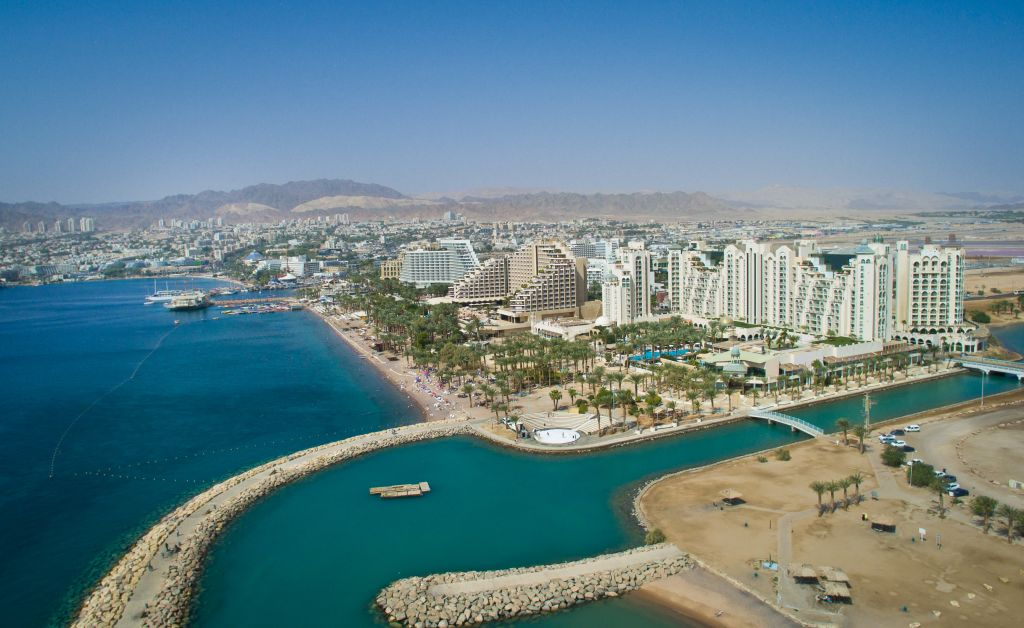
\includegraphics[width=1\textwidth]{images/eilat.jpg}
\end{center}
\vspace{0.5cm}

\begin{minipage}{0.45\textwidth}
    % Eilat logo & sponsor stuff
    \begin{flushleft} \large
        
\includegraphics[width=2.5cm]{images/eilat_logo.png} \\
        \textbf{Sponsored by:} \\
        A. Adamon, \\
        E. Toppel \\
        \textit{Eilat Municipality}
    \end{flushleft}
\end{minipage}
\begin{minipage}{0.45\textwidth}
    % WPI logo and advisor stuff
    \begin{flushright} \large
        \href{https://www.wpi.edu}{
\includegraphics[width=5.5cm]{images/WPI_logo.png}} \\
        \vspace{1.0cm}
        \textbf{Submitted to:}\\
        Professor Isa Bar-On
        \vspace{1.5cm}
    \end{flushright}
\end{minipage}
\newpage

% Begin preamble section of document; abstract is first
\pagenumbering{roman}
\begin{abstract}
    % Eilat is a city in southern Israel with a population of \textapprox50,000, but over 3 million tourists per year. The city suffers from severe congestion during commuting hours, with traffic jams along major city roads and backed up lines of cars waiting to enter the city by the highway in the north. This project aimed to aid Eilat city planners in their goal to improve Eilat transportation service offerings while minimizing environmental impact, and to investigate smart city technologies to reduce congestion. Research on smart cities was conducted, including case studies of other cities, listings of smart city tools, and their applications to Eilat. To further aid city planners in visualizing data, an extensible interactive website was created that displays mapping information and data on flights entering the region. Suggestions for services and citywide goals were developed to guide Eilat towards reducing congestion and becoming a smart city.
    
    Eilat is a city in southern Israel with a population of \textapprox50,000, \textapprox3 million tourists/year, and severe congestion. This project aimed to aid city planners in improving transportation services, minimizing environmental impact, and investigating smart city technologies. Smart cities research was conducted, including case studies, listings of technologies, and relevant analyses. An interactive website was created for planners, displaying transport and regional flight information. Suggestions for services and citywide goals were developed to reduce congestion and further smart city goals.
\end{abstract}
\newpage

% Generate table of contents, list of figures, and list of authorships
\tableofcontents\newpage
\listofauthorships
\listoffigures
\newpage

% Switch to regular page numbering, begin headers, switch to 1.5 line spacing
\pagenumbering{arabic}
\pagestyle{fancy}
\onehalfspacing

% Actual content begins here!
\section{Introduction}[All]\label{sec:intro}
Eilat is a city in the southern tip of Israel with a growing population of \textapprox50,000 and an area of 85 km$^2$. The city is a popular tourist destination, with over 3 million tourists per year from around the world. Given past trends, tourism is expected to continue increasing in the future. The city currently suffers from heavy congestion at peak hours, and the new Ramon airport on route 90 is expected to worsen the situation, increasing travel times. This compounded congestion will put a strain on Eilat's transport network, calling for an increased effort to shorten commute times, expand Eilat's transportation services, and streamline the travel experience. 

Currently, Eilat's public transport offerings are limited to taxis and intra-city buses operated by Egged. A bus ride from the west side of the city to the airport takes about 26 minutes with no traffic, and from Yotam Square to the Hotels zone is 35 minutes. These lengthy travel times are likely due to a high number of stops across a wide area. Strategically implemented policy changes, city restructuring, and connected technologies are proven to increase city efficiency.

Eilat's growing population and fluctuating tourism throughout the year have both placed strain on the existing transportation network, leading to heavy congestion. This project aimed to determine goals for Eilat's future transportation services by referencing other cities that have successfully tackled similar problems using smart city technologies. We worked to identify the gap between these cities' transportation network and Eilat's, to assist in better designing and allocating mobility services throughout the city while aiming to improve Eilat transportation's eco-friendliness. As part of that work we created a guide that consists of a goal-oriented timeline and an interactive website with maps and air traffic data to assist city planners and inform them on the results of our work.
 
\newpage
\section{Background}
Despite Eilat's population of only fifty thousand, its situation is complicated by congestion, the inefficiencies of the bus system, the influx of three million tourists every year, and future expansion plans.

\subsection{Eilat's Existing Transportation}
\subsubsection{Congestion}[Christopher M.]

\begin{figure}[H]
    \centering
    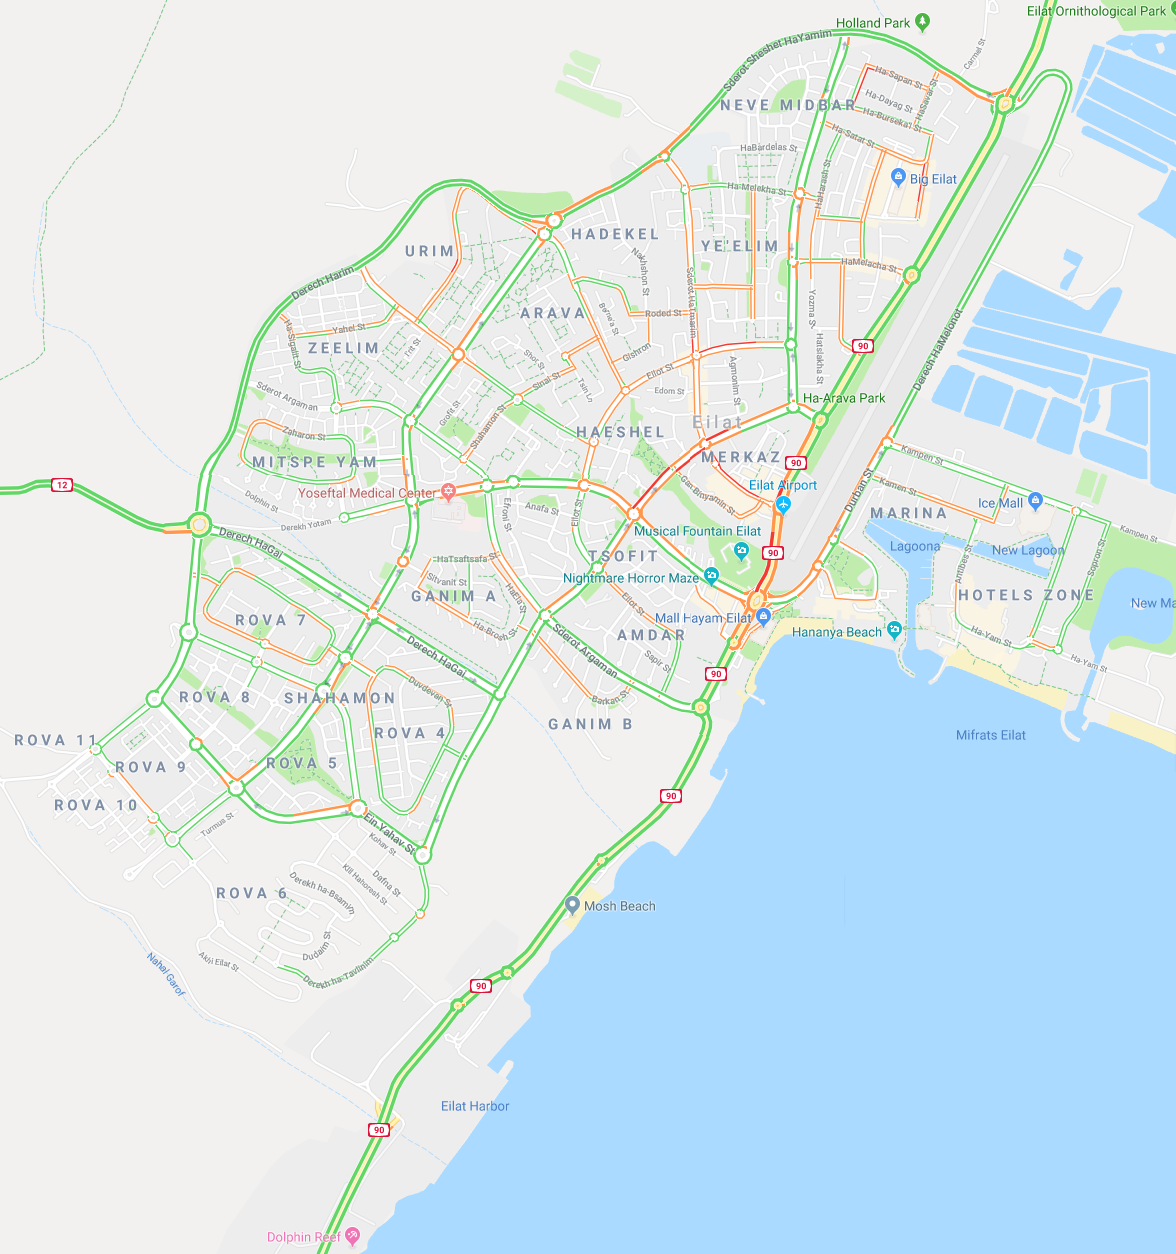
\includegraphics[width=0.8\textwidth]{images/eilat_traffic.png}
    \caption{Traffic map of Eilat at 5 PM weekdays (off-season)}
    \label{img:eilatTraffic}
\end{figure}

Israel's route 90 is the main road leading into Eilat, seen in the top right of figure \ref{img:eilatTraffic}, and is subject to heavy congestion during the tourism season, especially during peak hours. "Congestion" in the context of a road just means high density of cars on roads and resulting slowdowns; red and orange roads indicate heavy and moderate congestion, respectively. During rush hours congestion is moderate in most major city arteries, even off-season. A notable hotspot is the Eilat airport (on the center right) which travelers frequently enter and exit. However, this airport is set to shut down as Ramon Airport along route 90 sees more traffic, and Ovda Airport (which feeds into route 12 on the far left) will stop handling civilian flights. This leaves Ramon airport as the only airport servicing Eilat, enhancing the already-present focal point for congestion wherever route 90 meets with city roads. Commuting times see residents crowd on three major roads in the residential zone to the west as they move east to the industrial and commercial sectors of the city. The fact that three of Eilat's major schools are located along these roads only worsens congestion as parents drop off and pick up their children. Given current congestion, major traffic jams and long travel times can only be expected to increase.

\subsubsection{Private Vehicle Ownership}[Zachary Z., Valeria K.]
Private vehicles play a major role in the current state of congestion within Eilat. Based on data from our sponsors, it can be estimated that there are approximately 28,397 private cars on the roads today. This estimation assumes a similar modal split in transportation between 2013 and today, as well as a population growth rate that is congruent to the increase in private vehicle ownership over that span. Achieving a well-balanced split across transportation modes indicates that the services have been made equally convenient and tailored for various travelers. 56.5\% of people rely on private vehicles. The residents' affinity toward private-vehicles is clearly reflected in figure \ref{img:transportation_modal_split}, which shows the percentage of people in 2013 using each mode of transportation.

\begin{figure}[H]
    \centering
    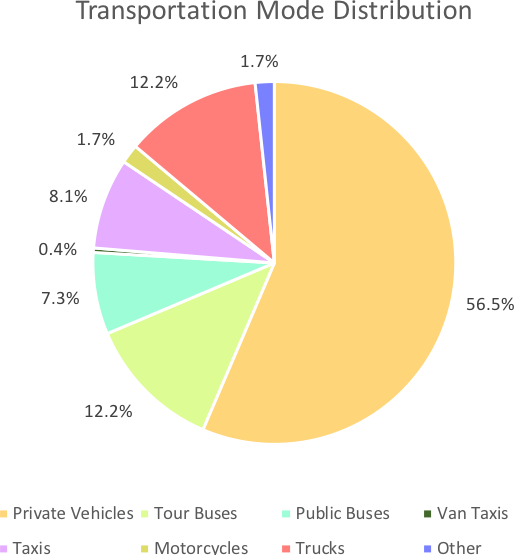
\includegraphics[width=0.5\textwidth]{images/transportation_distribution.png}
    \caption{Transportation Mode Distribution}
    \label{img:transportation_modal_split}
\end{figure}

(Aforementioned data provided by the sponsors of this project)

\subsubsection{Public Transit Design}[Evan. G]
Public transit uses several types of route structures to provide optimal service in an urban area \cite{Fielbaum2016OptimalStructure, WikiBooksFundamentalsWorld}:
\begin{itemize}
    \item \textbf{Radial routes} collect passengers from outlying areas and bring them to major areas (known as trip generators).
    \item \textbf{Cross-town (grid-like) routes} transport passengers across an area (sometimes between radial services or several smaller trip generators).
    \item \textbf{Direct connections} move passengers between major trip generators.
    \item \textbf{Circulators} collect and distribute passengers in smaller sub-areas.
\end{itemize}

An efficient transportation network typically features a combination of these types of routes. Bus systems in particular often include a combination of cross-town and radial routes, providing wide coverage as well as direct access to major destinations.

When laying out a route, the frequency of stops along the route (stop density) must be considered. The more stops along a route, the less passengers must walk to get to a bus stop; however, frequent stops results in a slower operating speed of the vehicle.

Another trade-off must be made between a route's coverage and its directness. A longer, more circuitousness route can collect passengers from a wider area, but also results in increased travel times compared to a more direct route covering a smaller area.

\subsubsection{Existing Bus System}[Evan G.]
Only 7.3\% of people in Eilat use the bus system, mostly out of necessity since the bus system is inefficient and inconvenient. Intra-city buses are operated by Egged. A bus ride across the city from the west to the hotel zone in the east takes between thirty and thirty-five minutes, while the same journey by car takes ten. Lengthy bus travel times are due to a large number of stops across a wide area for any given route.

The city of Eilat features a small number of major trip generators: the main beach and boardwalk, the hotel zone, and mosh beach by the dolphin reef. These areas are easily accessible from the commercial area in the city center and along route 90, but are difficult to access from the surrounding neighborhoods. As seen in figures \ref{img:bad_bus_1} and \ref{img:bad_bus_2}, these areas feature highly circuitous radial routes, but lack any direct routes or cross-town service. The only bus options from these areas into the city center is a very lengthy bus ride through multiple neighborhoods.

\begin{figure}[H]
    \centering
    \href{https://www.google.com/maps/dir/29.5578131,34.9388748/29.5512465,34.9536416/@29.5539541,34.9429944,15.12z/data=!4m2!4m1!3e3}{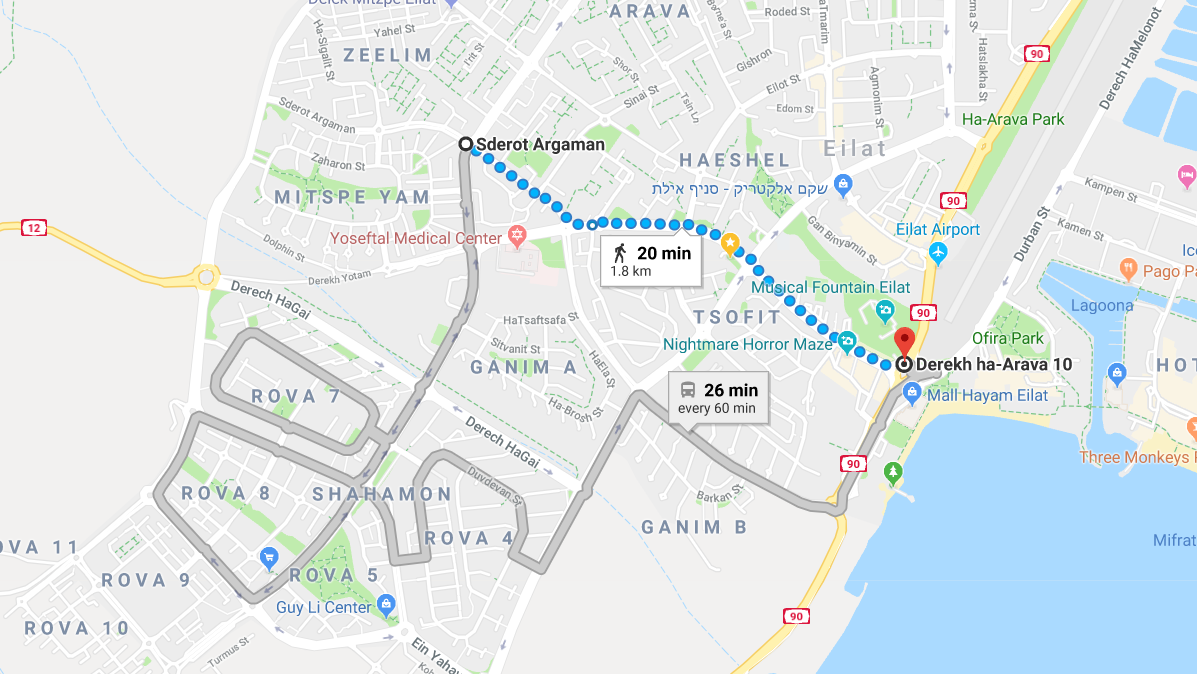
\includegraphics[width=0.65\textwidth]{images/bad_bus_1.png}}
    \caption{A radial route with no direct options}
    \label{img:bad_bus_1}
\end{figure}

\begin{figure}[H]
    \centering
    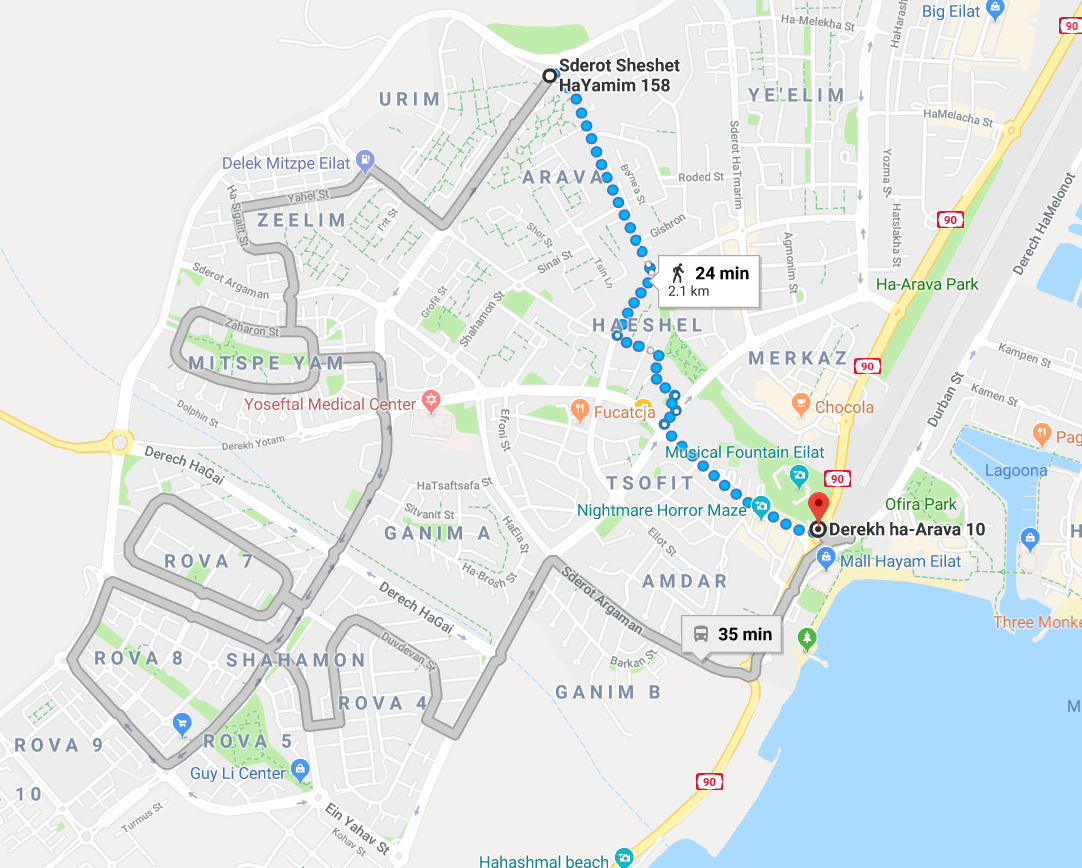
\includegraphics[width=0.65\textwidth]{images/bad_bus_2.png}
    \caption{A radial route with no direct options}
    \label{img:bad_bus_2}
\end{figure}

Figure \ref{img:bad_bus_3} demonstrates a situation where a direct route might be used to connect two trip generators (Mall Hayam and Mosh Beach), but no bus route exists.

\begin{figure}[H]
    \centering
    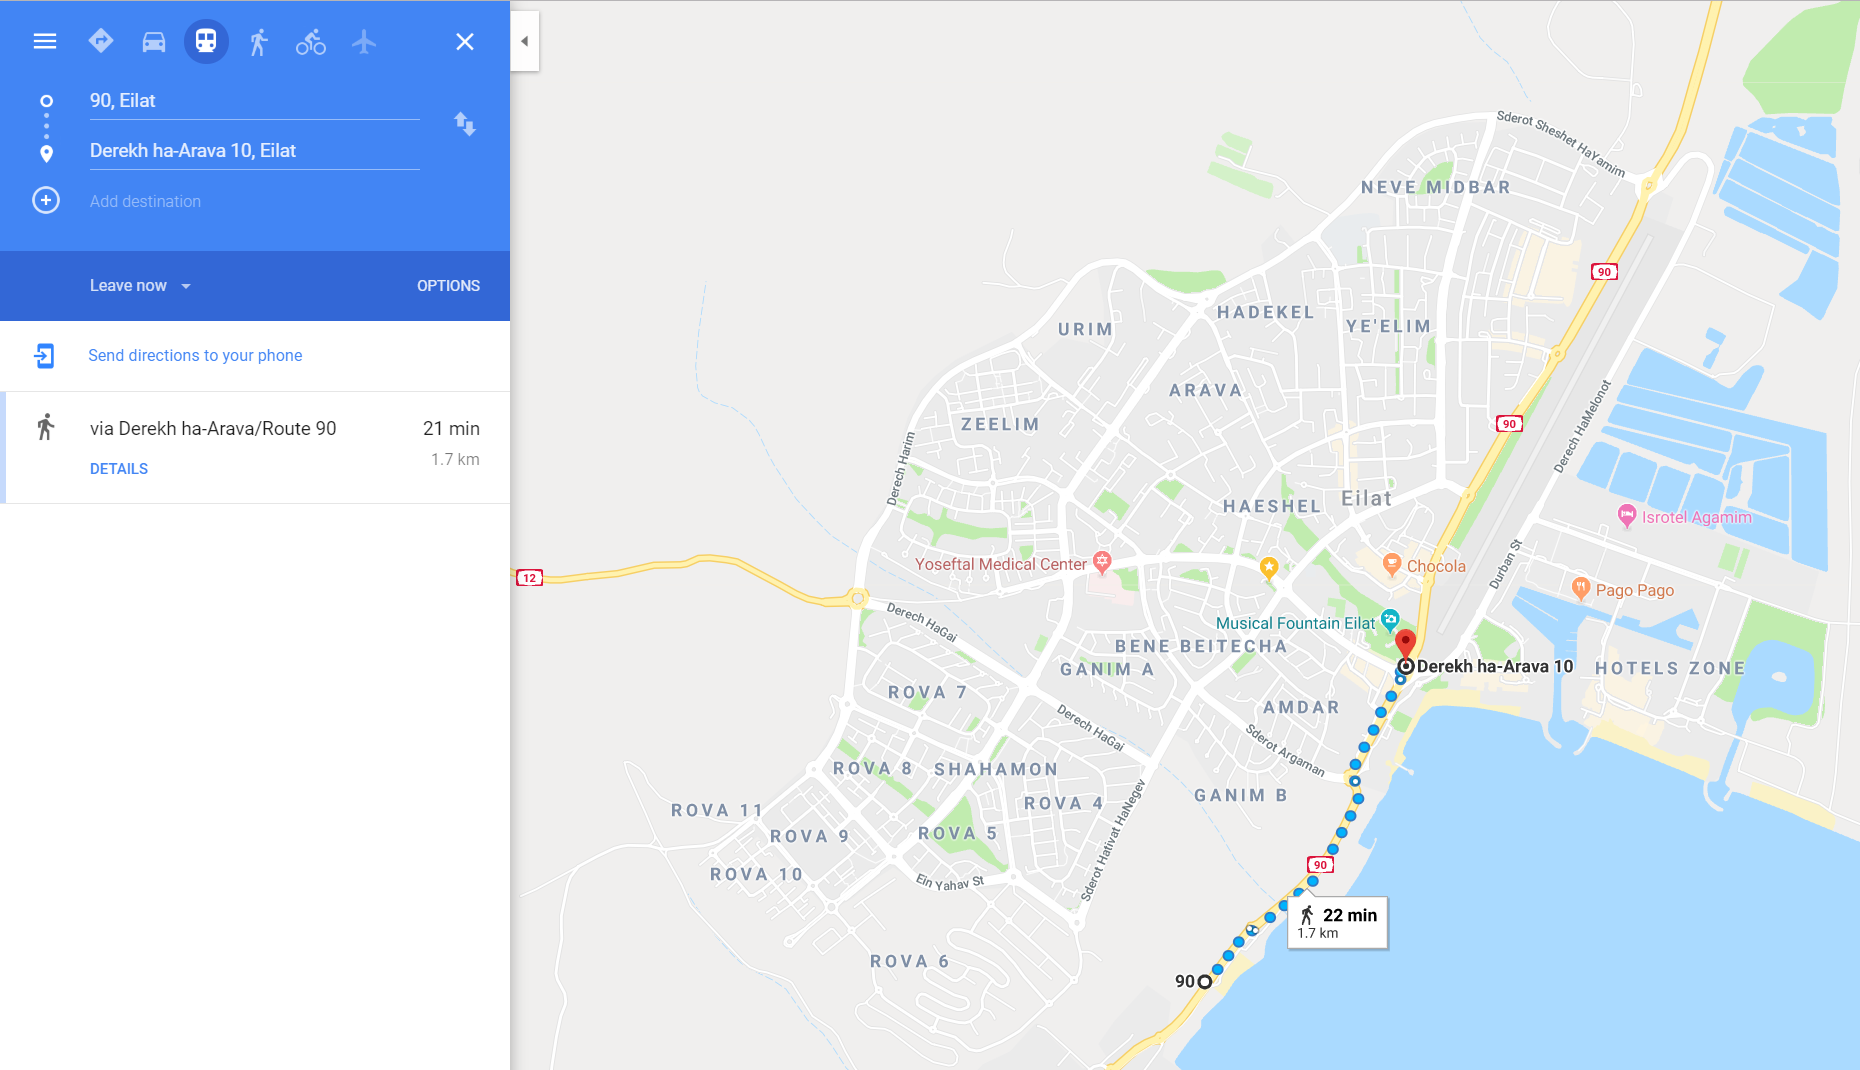
\includegraphics[width=1\textwidth]{images/bad_bus_3.png}
    \caption{No bus route available to Mosh Beach}
    \label{img:bad_bus_3}
\end{figure}

One of Eilat's primary transportation goals is to make public transportation as ecologically friendly as possible. The Egged fleet consists of diesel-powered buses, which do not fit with this goal. In 2017, Egged launched twenty-five electric buses in Haifa, and is currently assessing options for additional electric buses \cite{KerenKayemethLelsraelJewishNationalFund2017}.

User experience is an important factor in the use of public transportation. Moovit is the most popular public transportation app, providing information about expected arrivals of buses at a given stop in real time. Without the use of Moovit, it is difficult to predict when a bus will arrive at a stop. The app can only display Israel's bus information in Hebrew, making it difficult for international tourists to use.


\subsubsection{Parking}[Zachary Z.] \label{sec:parking}
The city has an existing parking system which can accommodate up to 4,241 vehicles at 100\% occupancy. The city plans to reduce the amount of parking by 2,334 spots within the next 4-5 years, leaving only 1,904 spots remaining. These lots are also mostly free parking, meaning the parking lots left over will be less enticing to use for drivers. 

Unsurprisingly, most of the parking lots were not at 100\% occupancy, with only 1,918 of the 4,241 (45.2\%) parking spots required to support the city's needs. If existing lots are not expanded, those in need of parking will spend more time on the roads. Avoiding this unnecessary car-traffic will mean increased considerations on real-time parking information, expansion of existing lots underground, and cost restructuring. 

In an effort to address non-resident private vehicles, Eilat has plans to construct a new parking lot northwest of Toronto square by 2020. This lot will have roughly 300 spots and provide a place for domestic tourists or outside commuters to drop off their cars to use the public transit from there on. To incentivize users, a shuttle will be available to give rides from the lot as far as southwest Eilat. This plan will concentrate more parking toward the outskirts of the city, presumably reducing the amount of private vehicles toward the center. 

(Aforementioned data provided by the sponsors of this project)com

\subsection{Eilat Tourism: Statistics and Demographics}[Valeria K., Zachary Z.]
Eilat's Red Sea beaches, coral reefs and marine life provide plenty of diving and snorkeling opportunities for tourists. The underwater observatory pulls people from all over and provides views of sharks, turtles, and rare fish \cite{Benner2017}. The musical fountain is a popular nighttime attraction, offering a unique audiovisual show to pair with the view of the city behind it. As a tax-free city Eilat is a major shopping center with five shopping malls within one square kilometer, the largest being Mall Hayam and the Ice Park Mall \cite{Benner2017}. These sites best serve families with children as they provide attractions for all ages and demographics. The city night life, including restaurants, bars, and clubs, makes it well-suited to young adults.

Domestic tourism is a major part of Israel's tourism industry, accounting for 90\% of hotel room occupation in Eilat \cite{Benner2017}. The Ministry of Tourism spends approximately 33\% of its budget on marketing, 28\% on investment incentives, and 26\% on infrastructure investment \cite{Benner2017}. The United States, Russia, France, the UK, and Germany account for nearly 50\% of international tourists. In 2012 Israel attempted to draw in more European and American tourists through an agreement with the European Union (EU) to allow direct flights between Israel and all EU countries \cite{Benner2017}. This agreement, called Open Skies, drove flight prices down and increased tourist flow to all parts of Israel. As of 2015, France and Russia represented the largest origin markets with a 42\% and 26\% claim respectively on international tourist arrivals Eilat, suggesting that Open Skies increased tourism pull from the EU \cite{Benevolo2016}.

In 2018 there were a total of about 6.5 million overnight tourists, of which approximately 89\% were Israeli tourists according to our sponsor. In 2018, hotel occupation was 73.2\%, or 11,034 hotel rooms.

From 2000 to 2018, Israelis account for the majority of Eilat's tourism at 87\%, whereas international tourists made up only 13\%. Figure \ref{img:historical_tourism_trends} shows an overview of tourism trends in Eilat from 2000 to 2018, and includes overall, international, and domestic overnight tourism. Domestic overnight tourism has shown a steady, slight increase. On the other hand, international overnight tourism has varied much more over the years. The overall trend of tourism most strongly resembles domestic tourism trends due to the drastically higher percentage of Israeli tourist. The distribution and trends of tourism are important to understand, due to the high volume of tourism Eilat experiences, and its strong influence on the city and its population. When considering the impact of tourism on congestion, keeping these divisions is relevant to, for example, which efficient modes of transportation are preferred by tourists especially how this can vary between domestic and international tourists.

\begin{figure}[H]
    \centering
    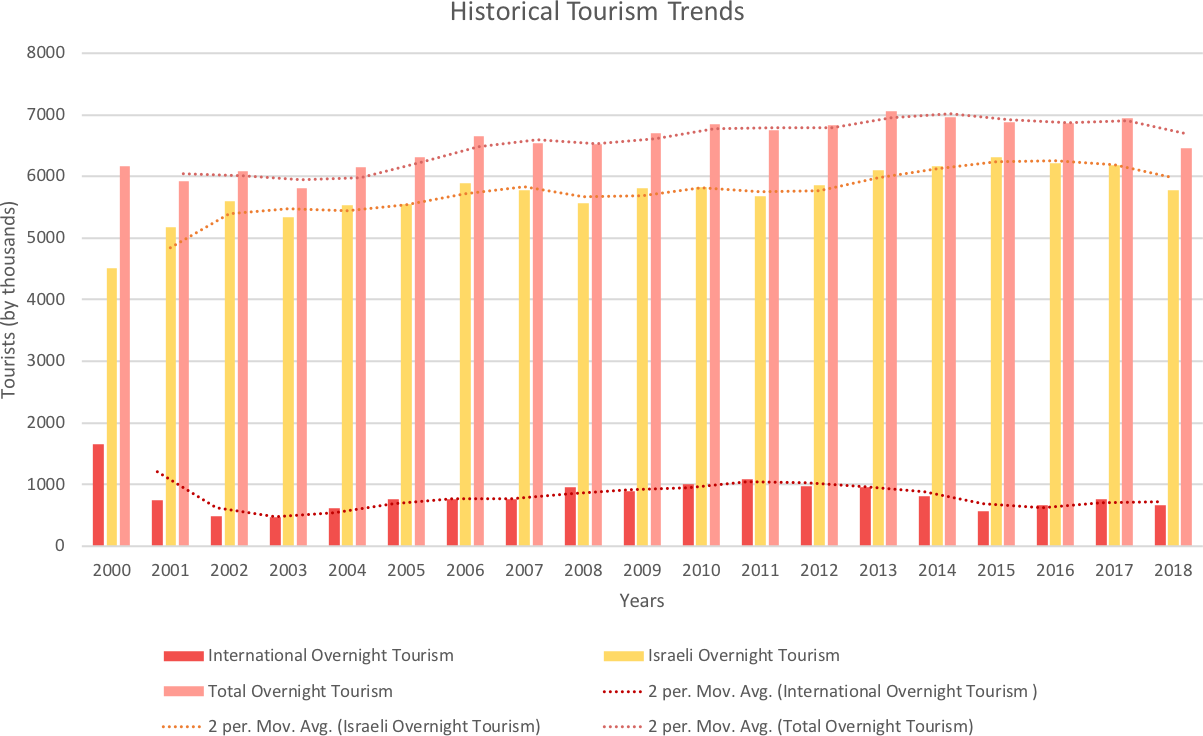
\includegraphics[width=1\textwidth]{images/historical_tourism_trends.png}
    \caption{Historical Tourism Trends}
    \label{img:historical_tourism_trends}
\end{figure}

Figure \ref{img:monthly_tourism} shows the overall overnight monthly tourism averages for the past three years (2016-2018). For this time period domestic tourism accounted for 89.6\% and the remaining 10.4\% was international. Eilat's peak tourism months are shown to be July and August. Keeping tourism variance in mind is important given that Eilat as a whole, especially in terms on congestion, changes greatly in response to the peaks and lows of tourism. 


\begin{figure}[H]
    \centering
    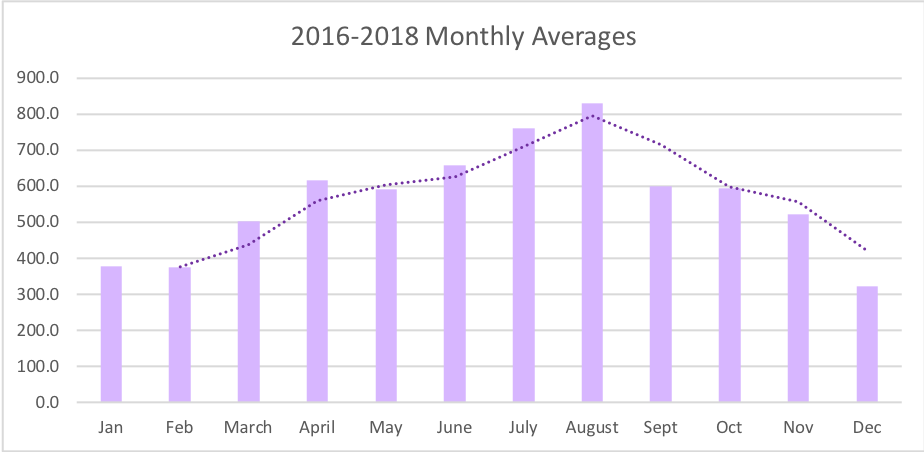
\includegraphics[width=1\textwidth]{images/monthy_tourism_averages.png}
    \caption{Monthly tourism averages}
    \label{img:monthly_tourism}
\end{figure}

The tourism monthly distribution is closely correlated to the monthly population density shown in figure \ref{img:monthly_population_density}. There is a peak in population density primarily around the summer months, at the same time tourism is at its highest.

\begin{figure}[H]
    \centering
    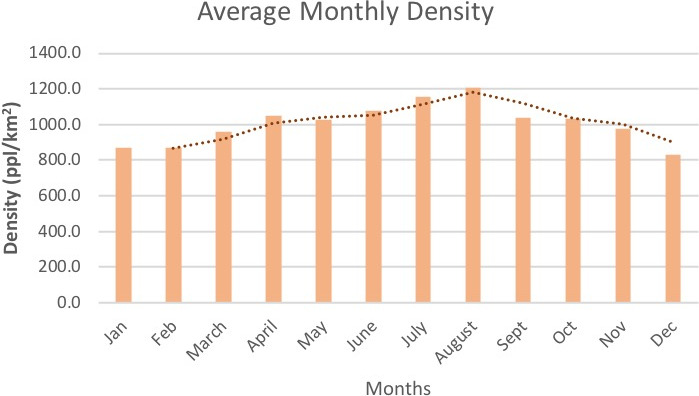
\includegraphics[width=1\textwidth]{images/monthly_population_density.jpg}
    \caption{Monthly population density in Eilat}
    \label{img:monthly_population_density}
\end{figure}

Though Eilat's population density is nominally at 600 ppl/km$^2$, the 3 million tourists per year play a major role in fluctuating it throughout the year. As seen above, the actual population density at any given time in a month is above 800 ppl/km, a 25\% increase. To calculate this, the percent split in tourist population by month (all summing to 100) was used to extrapolate how many tourists out of 3 million would come during each month. From here the length of the given month was divided by average length of stay in Eilat, 4.25 days, to obtain the average population density at any given point in a certain month \cite{IsraelMinistryofTourism2017}. All of these calculations were done in addition to the residents that are assumed to be constant (at 50,000) throughout the year. Sources of error in this lie in the assumption that these population densities are uniformly distributed throughout Eilat, when in reality they are concentrated most in tourist destinations and the center of the city. These areas would see much higher population densities, inherently causing more congestion in those areas. The issue of an ever-changing population, thus population density, is unique to Eilat in that most other cities don't experience populations with such high peaks and low troughs. Similarly to monthly tourism numbers, the variance in population density throughout the year and its correlation to congestion and increased stress on the city's resources are valid reasons to turn to smart city initiatives.

\subsection{Eilat Expansion and Zoning}[Valeria K., Zachary Z.]
% Figure \ref{img:eilat_zoning} shows Eilat's current layout and how it is zoned into residential, industrial, commercial and tourist areas. 

% \begin{figure}[H]
%     \centering
%     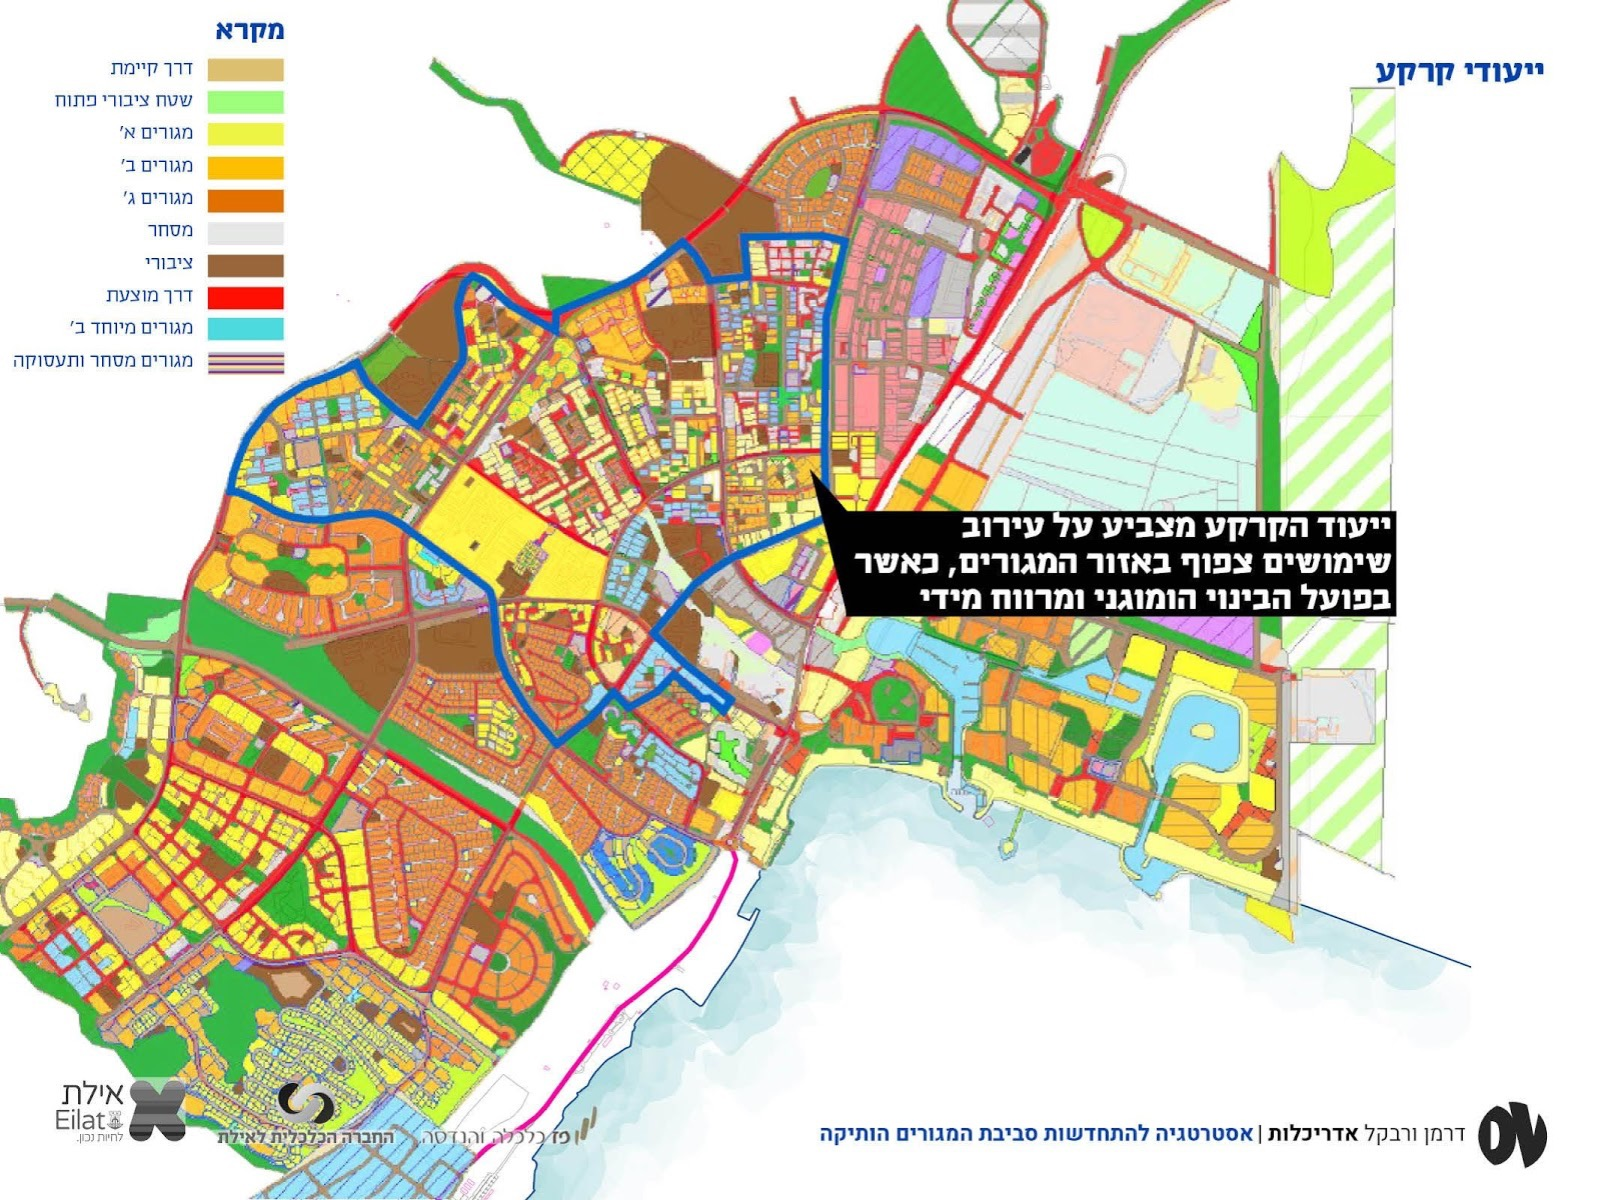
\includegraphics[width=0.7\textwidth]{images/eilat_zoning.jpg}
%     \caption{Map of Eilat zoning}
%     \label{img:eilat_zoning}
% \end{figure}

Residential areas in Eilat are divided into seven zones. Figure \ref{img:Residential_Age_Distribution} shows the average age distribution within these. 

\begin{figure}[H]
    \centering
    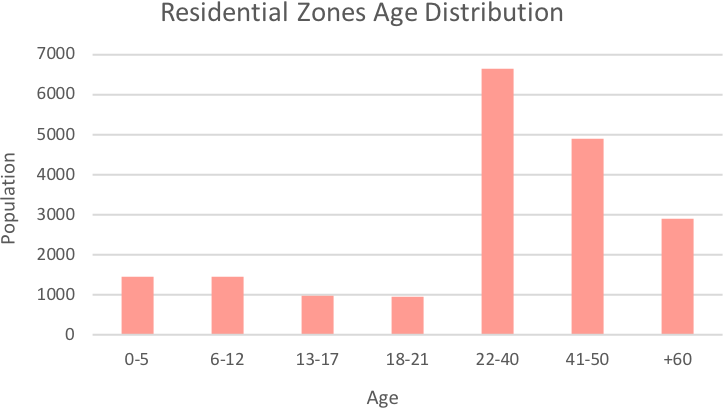
\includegraphics[width=0.8\textwidth]{images/resident_age_distribution.png}
    \caption{Residential Age Distribution}
    \label{img:Residential_Age_Distribution}
\end{figure}

This shows that the majority of Eilat's residents, accounting for 34.5\%, are between the ages 22 and 40. This is closely followed by residents between 41 and 50, at 25.4\%. The two subsets of the population make up the working demographic, given that the standard is that between ages 18 to 21 Israelis will traditionally do their military service. This means that 59.9\% of residents commute to work, presumably during similar hours in the mornings and afternoons, which coincide with peak traffic hours and worsen congestion.

% Figure \ref{img:eilat_expansion} shows future expansion plans for the city.

% \begin{figure}[H]
%     \centering
%     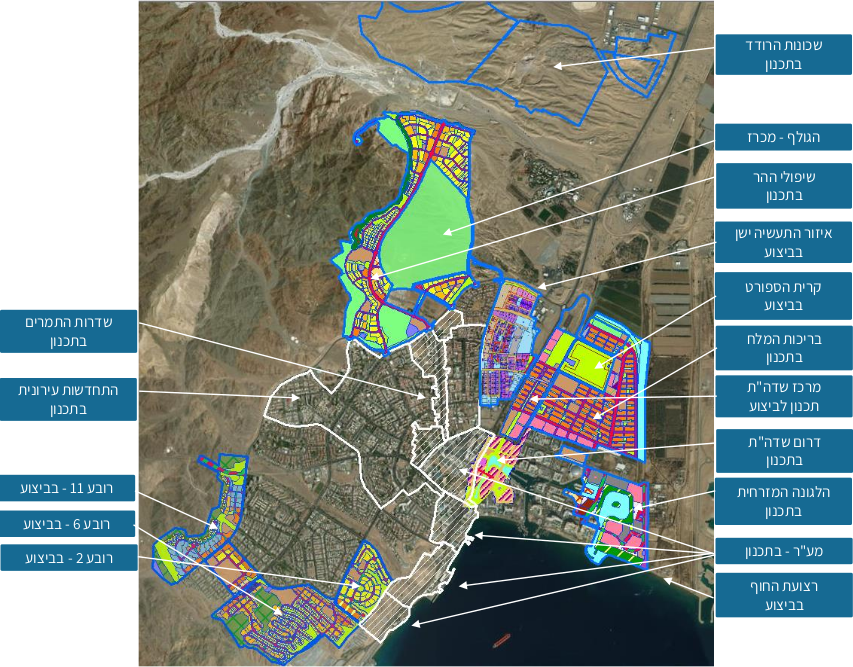
\includegraphics[width=0.9\textwidth]{images/eilat_zoning_future.png}
%     \caption{Map of future Eilat expansion \& zoning}
%     \label{img:eilat_expansion}
% \end{figure}

Eilat plans to expand the city significantly to the north by adding residences, hotels, and more tourist attractions, including a golf course. These additions will replace the existing airport in the city center, and currently unoccupied land toward the north and south-west. Removing the Eilat Airport will benefit the city, as the airport currently divides parts of the city and increases congestion in the Mall Hayam and Boardwalk area. This expansion would also alleviate some of the congestion that can be seen at peak airport arrival hours when taxis flood the area waiting to pick up travelers. Residents commuting to and from work during airport hours will face less traffic as a result, and services will concentrate toward the north. 

\newpage
\section{Smart Cities}\label{sec:smart_cities}
\subsection{Overview}[Valeria K., Zachary Z.]
Smart cities aim  to ease the lives of their citizens by providing efficient and convenient services, in part by analyzing data collected from sensors throughout the city. Cost, travel time, convenience, reliability, familiarity, weather, safety, environmental considerations, and existing infrastructure are factors that vary across cities and play a crucial role in understanding what citizens and visitors need and want \cite{CityofAustin2016}. This information can then be used to determine which services should be prioritized.

Existing smart city plans typically first incorporate a basic infrastructure of sensors, cameras, and city-wide WiFi in order to establish a constant stream of data. This data can be used in strategic ways to resolve the issues that are too dynamic and intricate to change via technology-neutral methods. These tools are installed through the city and collect data on traffic, available parking, pedestrian traffic, etc. This information can be used, for example, to improve traffic flow by adjusting public transportation and traffic lights to real-time demand.

Successful smart cities across the world have several common factors, such as strong commitments from government leaders that foster collaboration between the public sector and the private sector. Government transparency also greatly increases citizens' confidence and can be achieved by making collected data available. Additionally, prioritizing continuous improvement is crucial due to rapidly changing technologies, since smart cities need to be constantly evolving and adapting alongside them \cite{Zanghi2017WhyExamples}. 

Smart mobility (or mobility as a service) incentivizes customers with cheaper, faster, and more convenient modes of transportation than privately-owned vehicles. These services target issues associated with the saturation of private vehicles, such as traffic congestion, road accidents, insufficient parking, and greenhouse gas emissions.

\subsection{City Case Studies}[Valeria K.]
Detailed below are six examples of cities worldwide that addressed problems such as congestion and pollution. Influencing factors such as population, population density, climate, existing infrastructure, policy flexibility, and public opinion should be taken into account when considering proposed plans. It is important to note that these cities are all significantly larger, in terms of size and population, than Eilat. Relevant examples of successful implementations of smart cities and non-technological solutions to congestion were all best portrayed in cities of larger size, which is why the following were chosen despite their differences from Eilat. Each city established different goals, leading to various solutions and implementations, and studying these models provides valuable input for a model reflecting the services and transportation systems needed in Eilat.

\subsubsection{Curitiba, Brazil}[Valeria K.]
Curitiba is the capital of the state of Paraná in southern Brazil. With 1.8 million people, it is Brazil's 8\textsuperscript{th} most populous city, with about 2 million tourists per year \cite{Adler2016StoryCapital}. During the 1970s there were a series of projects that focused on improving the city after it experienced rapid growth leading to overly congested streets. These projects were led by architect and three time mayor Jaime Lerner. The first project, in 1972, converted the main street in the center of the city to a pedestrian mall. The public initially objected to this, especially shopkeepers. To bypass this, Lerner started construction on a Friday evening after the courts had closed and finished within seventy-two hours. Public opinion rapidly shifted when people saw the zone's benefits, and people supported further expanding the pedestrian zone. This was the beginning of an attitude change for Curitiba that focused on bringing people together. Lerner adopted a philosophy of "act now, adjust later" to avoid Brazil's bureaucracy, allowing the implementation of bold initiatives that would otherwise have been shut down or taken longer to carry out. Today, 85\% of the population uses the bus system, given that it is the fastest and cheapest mode of transportation in the city \cite{Adler2016StoryCapital}. The system, known as the Bus Rapid Transit (BRT), uses raised platforms and electronic prepayment that allows for quicker stops, features higher-capacity buses, and has five express bus avenues. The city has made an effort to have large green areas and has a widely adopted recycling program. Curitiba's successful implementation of its bold initiatives has brought it worldwide recognition as a model for urban planning.

\subsubsection{Freiburg, Germany}[Zachary Z.]
Freiburg, a city of about 220,000, suffered significant damage during World War II bombings, which led to a redevelopment of the inner areas during the reconstruction period. The population at the time prioritized their energy consumption and city layout, suggesting that a viable solution would focus on city access rather than private vehicles \cite{Rydningen2017}. Planners also decided to place emphasis on supporting diverse, cheap, and clean transportation modes and services \cite{Bindra2006}. Planners also considered air pollution due to traffic in the city center, and pedestrianized the center further to reduce the cars inside. This city center became a hotspot for tourists containing restaurants, shops, and plenty of green space. Parking is available outside the city center at a fee that increases progressively toward the center, reducing congestion \cite{Bindra2006}. The city first built an efficient tram system which, combined with the bus system, was able to bring travelers within 7 minutes of city outskirts. The city also made an effort to expand its biking network by placing bikes next to tram \& bus stations with parking available for cars \cite{Bindra2006}. From 1984 to 2006, public transit use doubled and a 9\% decrease of private vehicle usage for everyday travel needs indicated a modal shift. By 2020, Freiburg is projected to have 29\% of travelers using private vehicles, 20\% using public transit, 27\% using bicylces, with the remaining 24\% walking \cite{Rydningen2017}. Reducing the stress on any one form of transportation should contribute to a well-balanced city-wide network for all users. Figure \ref{img:freiburg_modal_split} reflects the current and projected usage of the transportation network in Freiburg.

\begin{figure}[H]
    \centering
    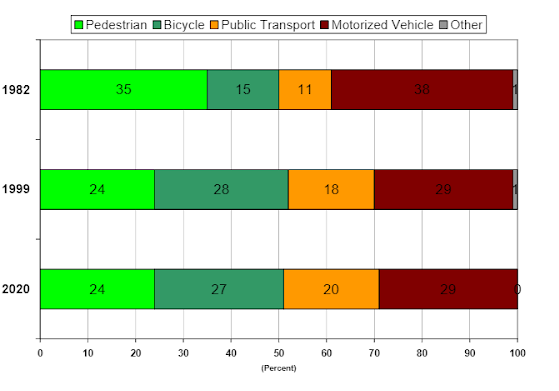
\includegraphics[width=0.9\textwidth]{images/freiburg_modal_split.png}
    \caption{Chart of Freiburg's transportation modal split over time.}
    \cite{Rydningen2017}
    \label{img:freiburg_modal_split}
\end{figure}

\subsubsection{Barcelona, Spain}[Valeria K.]
Barcelona is the second largest city in Spain with 1.7 million residents, and is one of the most densely populated European cities \cite{Bausells2016}. It a popular tourist destination in Europe, with about 8.2 million international visitors per year \cite{Bausells2016}. Barcelona is widely recognized for its smart city initiatives that stemmed from its need to address high levels of air pollution (well above the threshold established by the European Union). The city has successfully implemented various smart city technologies, such as sensors that measure air quality, street lights that dim when there are no pedestrians in the area, and sensors in public parks to decrease unnecessary water usage. The city boasts a smart bus system with increased routes and with smart bus stops that include free WiFi, charging stations and real life time updates of the bus schedule. It has an extensive bike-sharing program with about 180 km of bicycle lanes. The metro system is 1.5 km per hour faster than the average car trip within the city \cite{Bausells2016}. In order to decrease air pollution, Barcelona will ban cars made before 1997, and trucks \& vans made before 1994. Additionally, Barcelona is now implementing a plan to establish "superblocks" through out the city. These are areas that encompass about nine blocks and prioritize pedestrians. Cars can circulate within the superblocks, but they have to do so at slow speeds, which will ideally lead to cars staying mostly within main roads and traffic flowing around them. Overall, the superblocks aim to foster communities and increase life quality. Figure \ref{img:barcelona_superblock} shows a comparison of the current city layout and the proposed layout structure of superblocks.

\begin{figure}[H]
    \centering
    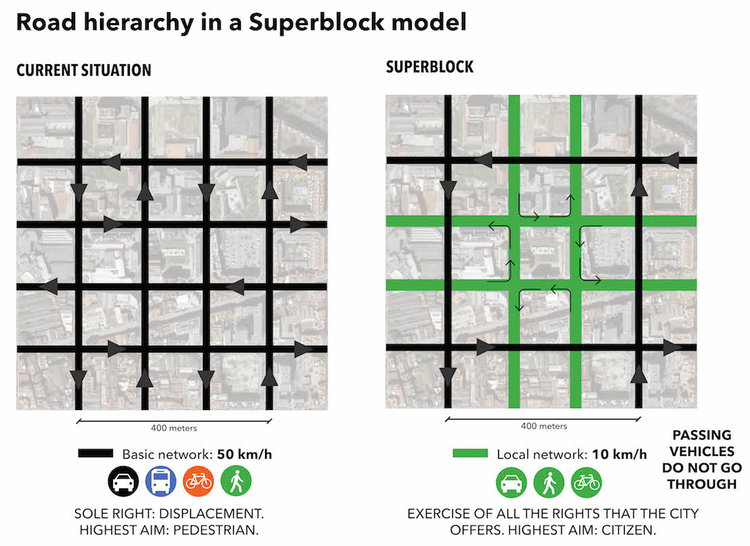
\includegraphics[width=0.85\textwidth]{images/barcelona_superblock.jpg}
    \caption{Diagram of Barcelona's "superblocks"}
    \cite{Streetfilms2018}
    \label{img:barcelona_superblock}
\end{figure}

\subsubsection{Kansas City, United States}[Zachary Z.]
The Smart City Challenge asked mid-sized cities (definitions of mid-sized cities vary) across the United States to provide a plan for moving to a brand-new transportation system that would "use data, applications, and technology to help people and goods move more quickly, cheaply, and efficiently" \cite{CityofDenver2016}. Given Kansas City's existing strengths and policymakers, they had achievable goals to create a higher quality of life, reduce traffic, through interconnected smart technologies. At the time of the challenge, having the most highway miles in the region and the most established infrastructure of fiber optics and WiFi in the country was one of Kansas City's most valuable assets. These resources eliminated the need to build a network from scratch, unlike many other cities. The city also emphasized the use of bikes by implementing road diets and including a way-finding app for bikers called RideKC. Though this was a start, Kansas City had 3 different plans in their Smart City + Connected City proposal. Their plan entailed making improvements to underdeveloped areas in the east side, introducing autonomous and connected vehicle technologies, as well as increasing connectivity sharing throughout the city. To address the east side, they added a 3.5 km tram line which allowed easier transport to the center and east side. They also added new way-finding apps for pedestrians, and planned to increase their offerings for ride-sharing and bike-sharing. In addition they began pilot tests for autonomous vehicles in a main artery within the city to test the viability of it expanding. These vehicles will also be connected to events, traffic, and could be implemented slowly while the infrastructure and policy-making develops. The city also plans to partner with cellular and ridesharing companies to obtain important real-time data, further expand the WiFi network to gather user data, and install information kiosks for travelers \cite{CityofDenver2016}.

\subsubsection{Singapore}[Zachary Z.]
Singapore has a population of 5.6 million, or nearly 8,000 people per square kilometer, and is expected to grow to 6.9 million by 2030 \cite{SingaporeLandTransportAuthority2016}. The city believes it can use its technology-based economy and infrastructure to its advantage to combat the anticipated increase in density. First, the city will make itself more pedestrian and biker-friendly by providing more bike lanes and pedestrian mobility services. Using autonomous cars, the city hopes to implement Mobility as a Service (MaaS) and reduce the amount of private vehicles on the road \cite{Huiling2017}. Though autonomous cars are difficult to test in a place with such a significant population density, it would alleviate major congestion areas and reduce accidents, commute times, and allow for vehicle-to-vehicle (V2V) communications. Data gathered from these autonomous vehicles, cameras, sensors, and people on the city-wide network will be analyzed and redistributed to vehicles and travelers to adjust to real-time issues within the city \cite{SingaporeLandTransportAuthority2016}. This system would save people money, time, and would make it easier for users to pay. Since vehicles take up 12\% of the city's area, we can assume that constantly moving autonomous cars would significantly increase the amount of available city land previously held by parked private vehicles \cite{Huiling2017}. Though Singapore has lofty goals, they hope to achieve full autonomous fleets in the next 10 to 15 years.

\subsubsection{Columbus, United States}[Valeria K.]
In 2015 Columbus, Ohio won the Smart City Challenge created by the U.S. Department of Transportation (DOT), which resulted in a \$50 million grant given to fund the city's plans to create a smart transportation system \cite{GovernmentTec2016}. The city raised an additional \$500 million from mostly the private sector to support further smart technologies, such as funding autonomous vehicle testing. The collaboration between the public and private sectors has been crucial in Columbus's success in implementing its plan to transition into a smart city. It has installed sensors throughout the city that work to allow integrated data exchange (IDE) in order to decrease congestion and smooth transportation. For example, this allows emergency vehicles to interact with traffic lights to decrease travel time. Columbus aims to convert to EVs and wants to decarbonize the city's electric grid. It is also testing autonomous vehicles and created a playbook in order to share projects, case studies, and strategies with other cities looking to implement smart city technologies.

\subsubsection{Table of Cities}[Valeria K., Zachary Z.]
\begin{table}[H]
    \centering
    \singlespacing
    \small
    \begin{tabular}{ m{0.12\textwidth} | m{0.07\textwidth} | m{0.11\textwidth} | m{0.16\textwidth} | m{0.19\textwidth} | m{0.19\textwidth} }
        \textbf{City} & \textbf{Pop.} & \textbf{Density} & \textbf{Problem} & \textbf{Goal} & \textbf{Plan} \\
        \hline{}
        Curitiba, Brazil &
        1.76M &
        4,062/km$^2$ &
        \begin{flushleft}Rapid population growth led to high congestion \end{flushleft} &
        \begin{flushleft}Provide better quality of life and transportation for citizens\end{flushleft} &
        \begin{flushleft}Pedestrian city center, bus rapid transportation, biking lanes, and green areas\end{flushleft} \\ 
        \hline{}
        
        \flushleft Freiburg, Germany &
        227K &
        1,500/km$^2$ &
        \begin{flushleft}Reconstruction after WWII \end{flushleft} &
        \begin{flushleft}Move away from car predominance, prioritize pedestrians\end{flushleft} &
        \begin{flushleft}Pedestrian city center, extend \& improve bike network, expand tram \& bus lines\end{flushleft} \\
        \hline{}
        
        \flushleft Barcelona, Spain &
        1.6M &
        16,000/km$^2$ &
        \begin{flushleft}High noise \& air pollution, saturated streets\end{flushleft} &
        \begin{flushleft}Move away from car predomincance, prioritize pedestrians\end{flushleft} &
        \begin{flushleft}Mini-superblocks, repurpose existing infrastructure, bike lanes, orthogonal bus network\end{flushleft} \\
        \hline{}
        
        \flushleft Kansas City, US &
        489K &
        1,472/km$^2$ &
        \begin{flushleft}Underdeveloped regions in the city, outdated/ underutilized transportation\end{flushleft} &
        \begin{flushleft}Improve mobility and quality of life for citizens, reduce traffic, and create a smart city\end{flushleft} &
        \begin{flushleft}Use fiber optics and WiFi to gather user data, AV/CVs to provide a ride service, information kiosks \end{flushleft} \\
        \hline{}
        
        Singapore &
        5.6M &
        7,909/km$^2$ &
        \begin{flushleft}High density \end{flushleft} &
        \begin{flushleft}Reduce private vehicles \end{flushleft} &
        \begin{flushleft}Autonomous taxis, data collection, improve ease of use\end{flushleft} \\
        \hline{}
        
        Columbus, Ohio &
        879K &
        1,552/km$^2$ &
        \begin{flushleft}Worsening congestion\end{flushleft} &
        \begin{flushleft}Improve public transportation, Convert to EVs, testing for autonomous vehicles\end{flushleft} &
        \begin{flushleft}Partner with the private sector, Integrated Data Exchange (IDE), smart city technologies\end{flushleft}
    \end{tabular}
    \caption{Table of smart cities}
    \label{tab:smart_cities}
\end{table}

\subsection{Applications for Eilat: Advantages and Disadvantages}[Valeria K., Zachary Z.]
These case studies of cities show general trends in what solutions are being used to address similar problems to those faced by Eilat. These cities serve as examples that range from smart city proposals and successful implementations to cities that tackled problems, such as congestion, through other more technology-neutral solutions. Comparing these to Eilat's characteristics is useful in understanding what could be implemented in Eilat, what constraints would be present, and how these can be adapted to Eilat. Two factors that are key and vary greatly between Eilat and the city case studies are population density and size. Eilat is a much smaller city than all of the aforementioned cities and consequently has a lower population density, even during tourism peaks. This will greatly influence which suggestions make sense when applied to Eilat. It does not discount them; however, these need to be tailored specifically to Eilat's distinct characteristics. The extreme heat during summertime in Eilat also arises multiple times, and the high tourism fluctuation should also be taken into consideration. Through this scope the following advantages and disadvantages can be taken into consideration in regard to applying similar approaches to Eilat. 

Curitiba and Freiburg both implemented a pedestrian city center, eliminating congestion within. Eilat's city center, unlike those of these two cities, is not concentric, which means that determining what zone to pedestrianized is more complicated. The location of the Eilat Airport also poses an obstacle to developing a pedestrian center; however, given that this area will be repurposed in the coming years this is only a temporary constraint. An alternative to this is to extend the existing boardwalk along the water. This also helps address the extreme heat during the summer months. The sea provides a chilling factor that will encourage people to walk outside, whereas an otherwise pedestrian city center might not be as effective as it has been in other cities with milder climates. Curitiba was very intentional about creating green spaces in the city, and this could be greatly beneficial for Eilat since it would improve quality of life for residents and would be appealing for tourists. Including green spaces within or in conjunction to a pedestrian center. Additionally, most of the studied cities made a conscious effort to promote cyclists by having bike sharing programs. Road diets contribute to this by reducing the size of the roadways to prioritize room for bike paths and pedestrian walkways. According to Eilat city planners, the mayor of Eilat aims to promote a healthier and more active lifestyle for Eilat's residents. Adjusting infrastructure in the city and offering services to promote walking and cycling is in the city's best interest to accomplish this and decrease congestion. Once again, Israel's climate must be taken into account and providing more shade throughout the city would further help address this issue. 

Investing in the improvement of public transportation has been incredibly beneficial to multiple cities such as Curitiba, Freiburg and Barcelona. Having transit stops placed throughout the city so that citizens do not have a long transition from wherever they are located to the nearest stop has been key. Barcelona has much higher population density than Eilat, which is why it implemented both a metro system \textbf{and} a bus system. Eilat's lower population density, even during tourism peaks, means that this is not necessary. Focusing on the improving the existing bus system is a better allocation of resources. Curitiba chose to focus on developing its bus system, which more closely resembles the efforts Eilat should strive towards. Making sure waiting times are short is an important factor these cities emphasized, and is especially important for Eilat due to high summer heat. 

Barcelona's superblocks plan is aimed at a much larger city with a higher population density and higher pollution levels. This means that in order to implement it in a smaller city such as Eilat it would need to adapt to a much smaller scale. Perhaps a more practical approach would be to take specific characteristics of the superblock model and incorporate these into Eilat, and discount others that are not applicable. For example, the nine-block structure typical to superblocks in Barcelona would not be a logical implementation in Eilat. Instead the superblocks would most likely need to be designated areas, that are not strictly composed of a block formation. Other key components of superblocks can still be implemented in Eilat. Focusing on the idea of forming areas where traffic is discouraged (unlike the pedestrian center there is no traffic) in a way that traffic flows around it could be beneficial. This would likely be most useful in residential areas and the hotel area. This provides an alternative to completely blocking off cars, but still prioritizing pedestrians in the area. Barcelona chose to gradually re-purpose existing infrastructure to establish the superblocks instead majorly restructuring, providing a smoother transition for residents, which is a form of implementation that would likely work in Eilat as well. 

Singapore is an example of a city which strategically tackled its issues with its strengths in mind. Though the technology needs to develop, the city has a conducive environment for testing new technologies, both because of progressive policy makers and residents, and significant infrastructure already exists. Relating this to Eilat, it is clear that a target of implementing autonomous vehicles in the next 10 years is impractical given the lack of infrastructure. This being said, it should be noted that nearly every smart city required cameras and sensors, an extensive WiFi network to gather real-time information, and accessible resources for travelers to explore, book, and pay for transportation. This would be step one for Eilat in moving toward a technologically-oriented smart city that adapts to the unique needs of its citizens as well as its many tourists. It can be said that Singapore suffers from fundamentally different issues than Eilat and has a largely different geographic situation (climate, topography, regional location); however, Eilat does suffer from relatively high population density at times of peak tourist season. 

It is important to see the way other cities address their problems from the perspective of their approach, process, and ultimate resolution. Eilat's problems are unique to itself in that the factors that play into creating a tailored solution vary throughout the year. The drastic differences between mild winters and scorching summers, and between high and low tourist seasons require that any solution be adaptable. Smart city plans can address these fluctuations when deployed and maintained effectively.

\subsection{Cities that continue to struggle with congestion}[Valeria K.]
London and San Francisco are both large cities with high population densities and high levels of congestion. Both have attempted to address congestion without overall successful results. 

London implemented a congestion charge in the city center 15 years ago. This initially resulted in a big drop in congestion in the area of about 25\% \cite{Badstuber2018LondonIt}; however, this strategy is experiencing a plateau. Congestion in the city center has increased again, with long travel times, and high usage of private vehicles. There are several factors that have contributed to the increasingly high use of private vehicles such as the fact that the bus system is considerably slow; therefore, most people do not use it. Additionally, delivery services and private vehicles for hire are unregulated and seriously contribute to the cars that circulate within the city center. Some believe that bicycle lanes simply slow down cars and are not contributing to improving the situation. London is currently looking to change the congestion charge from a flat fee to a charge based on when and where drivers enter the charge zone and for how long they stay in it. They are also planning on expanding the zone and implementing a hierarchical structure for car prioritization within the city center, so emergency vehicles will be given top priority. 

Between 2010 and 2016 San Francisco's population increased by 70,000 people and 150,000 new jobs were created \cite{Marshall2018UberComplicated}. This led to a rapid increase in congestion, with 30\% of it being attributed to parking \cite{Marshall2018UberComplicated}. Private vehicles for hire, such as Uber and Lyft, as well as service delivery are being blamed for making existing congestion worse. Despite 32\% of its residents using public transportation the city continues to struggle with heavy congestion \cite{Marshall2018UberComplicated}. It is currently striving towards alleviating congestion by transitioning into a smart city; however, tangible progress is yet to be achieved. 

\subsection{Smart City Tools} 
\subsubsection{Sensors}[Valeria K., Zachary Z.] \label{sec:smart_city_sensors}
A key component of smart cities are interconnected technologies that rely on sensors that collect data. This data is analyzed in real time and allows for immediate changes that result in improvements. The following lists the most common and useful sensor-based technologies found in smart cities world wide. 

\begin{table}[H]
    \centering
    \small
    \begin{tabular}{l|l}
        \textbf{Technology} & \textbf{Use} \\
        \hline{}
        
        Parking sensors &
        Detect available parking, report \& pay w/app \\
        \hline{}
        
        Traffic-light sensors &
        Track \& dynamically adapt to traffic \\
        \hline{}
        
        Connected cameras &
        Capture traffic, crime, crowd data \\
        \hline{}
        
        Street-light sensors &
        Dim lights when unneeded \\
        \hline{}
        
        Open data platform &
        Share collected data, allow third-party analysis \\
        \hline{}
        
        Water sensors &
        Reduces water usage in parks \\
        \hline{}
        
        Municipal WiFi &
        Allow internet connections anywhere
    \end{tabular}
    \caption{List of smart city sensors \& data acquisition technologies}
    \label{tab:smart_city_sensors}
\end{table}

\subsubsection{Services}[Valeria K., Zachary Z.] \label{sec:smart_city_services}
\begin{table}[H]
    \centering
    \small
    \begin{tabular}{l|l}
        \textbf{Technology} & \textbf{Use} \\
        \hline{}
        
        Smart public transit &
        Adjusts city's supply to real time needs \\
        \hline{}
        
        Shared shuttles &
        Point-to-point group ridesharing \\
        \hline{}
        
        Ride-sharing &
        Private on-demand 'taxis' with pre-calculated cost \\
        \hline{}
        
        Bike-sharing &
        "Last mile" solution of bike rental through an app \\
        \hline{}
        
        Smart hubs &
        Digital kiosks that provide services \\
        \hline{}
        
        Car e-rentals &
        Cars available for easy rent online \\
        \hline{}
        
        Streetcar/subway system &
        Light trains on rails in the streets or underground \\
        \hline{}
        
        Bus system &
        Private or public buses with stops in the city \\
        \hline{}
        
        SkyTran &
        Above-ground rail system with users in pods \\
        \hline{}
        
        Autonomous vehicles &
        Computer-controlled cars, still experimental \\
        \hline{}
        
        Taxis &
        Traditional ride-costed taxi services \\
        \hline{}
        
        E-scooters/E-bikes &
        "Last-mile" solutions with distance/time rates \\
        \hline{}
        
        Carpool &
        Group travel in one car \\
        \hline{}
        
        Online payment &
        Payment through app
    \end{tabular}
    \caption{List of smart city services}
    \label{tab:smart_city_services}
\end{table}

\subsubsection{Additional Technologies}[Valeria K., Zachary Z.]
\begin{table}[H]
    \centering
    \small
    \begin{tabular}{l|l}
        \textbf{Technology} & \textbf{Use} \\
        \hline{}
        
        EV charging stations &
        Charging stations for electric vehicles \\
        \hline{}
        
        V2X communications &
        Vehicle-to-any [connected device] communications
    \end{tabular}
    \caption{List of misc. smart city technologies}
    \label{tab:additional_tech}
\end{table}

\subsubsection{Policies}[Valeria K.] \label{sec:policies}
An important aspect of decreasing congestion and improving citizen quality of life is implementing policy changes. There are various city policies that have been designed specifically for this purpose and used in various cities through out the world. One of these is congestion pricing, in which there is an imposed fee for entering a zone, typically the city center or the most congested area in the city. Some cities implement a fixed fee, such as London. Other cities have a fee that reflect the current congestion, when/where a vehicle is entering the zone and how long it is staying in it.

Another policy that has been implemented in cities such as Florence, Italy is restricted traffic zones. This is used when a city is divided into zones that are closed to traffic in varying levels. Access to zones can be determined in several ways, such as by time periods throughout the day/week, an entry-level based subscription, tiered fees based on proximity to center (number of cars inside), and plate number restrictions. Car entry can also be limited to residents, taxis, and emergency vehicles within designated zones, such as the city center. 

Parking restrictions are also oftentimes implemented to address congestion. There are multiple ways to implement parking restrictions such as imposing a parking ban within the city center and having available parking outside of it. Having parking become incrementally pricier closer to the city center is another method. This can also be tied to the parking sensors that indicate real-time parking suggestion through an app.

Speed reductions in the form of severe reduction of speed limits within specific areas, as seen in superblocks in Barcelona, serve to accommodate bikers and pedestrians. It also discourages car usage within that area. Additionally, road diets can be used to reduce the available vehicle driving space on roads to make bike lanes and pedestrian walkways available.


\newpage
\section{Interactive Map Website}\label{sec:site}
\subsection{Overview}[Christopher M.]
To gain a better understanding of transportation within the city, an interactive mapping \& general transportation website was developed. The site is not intended to be used by Eilat citizens or tourists, but instead contains information on Eilat traffic patterns, location of buses and their stops, city zoning information, and data on flight arrivals to the three airports that service Eilat. This site represents the first iteration of a tool that city planners will find useful, which they previously did not have.

\begin{figure}[H]
    \centering
    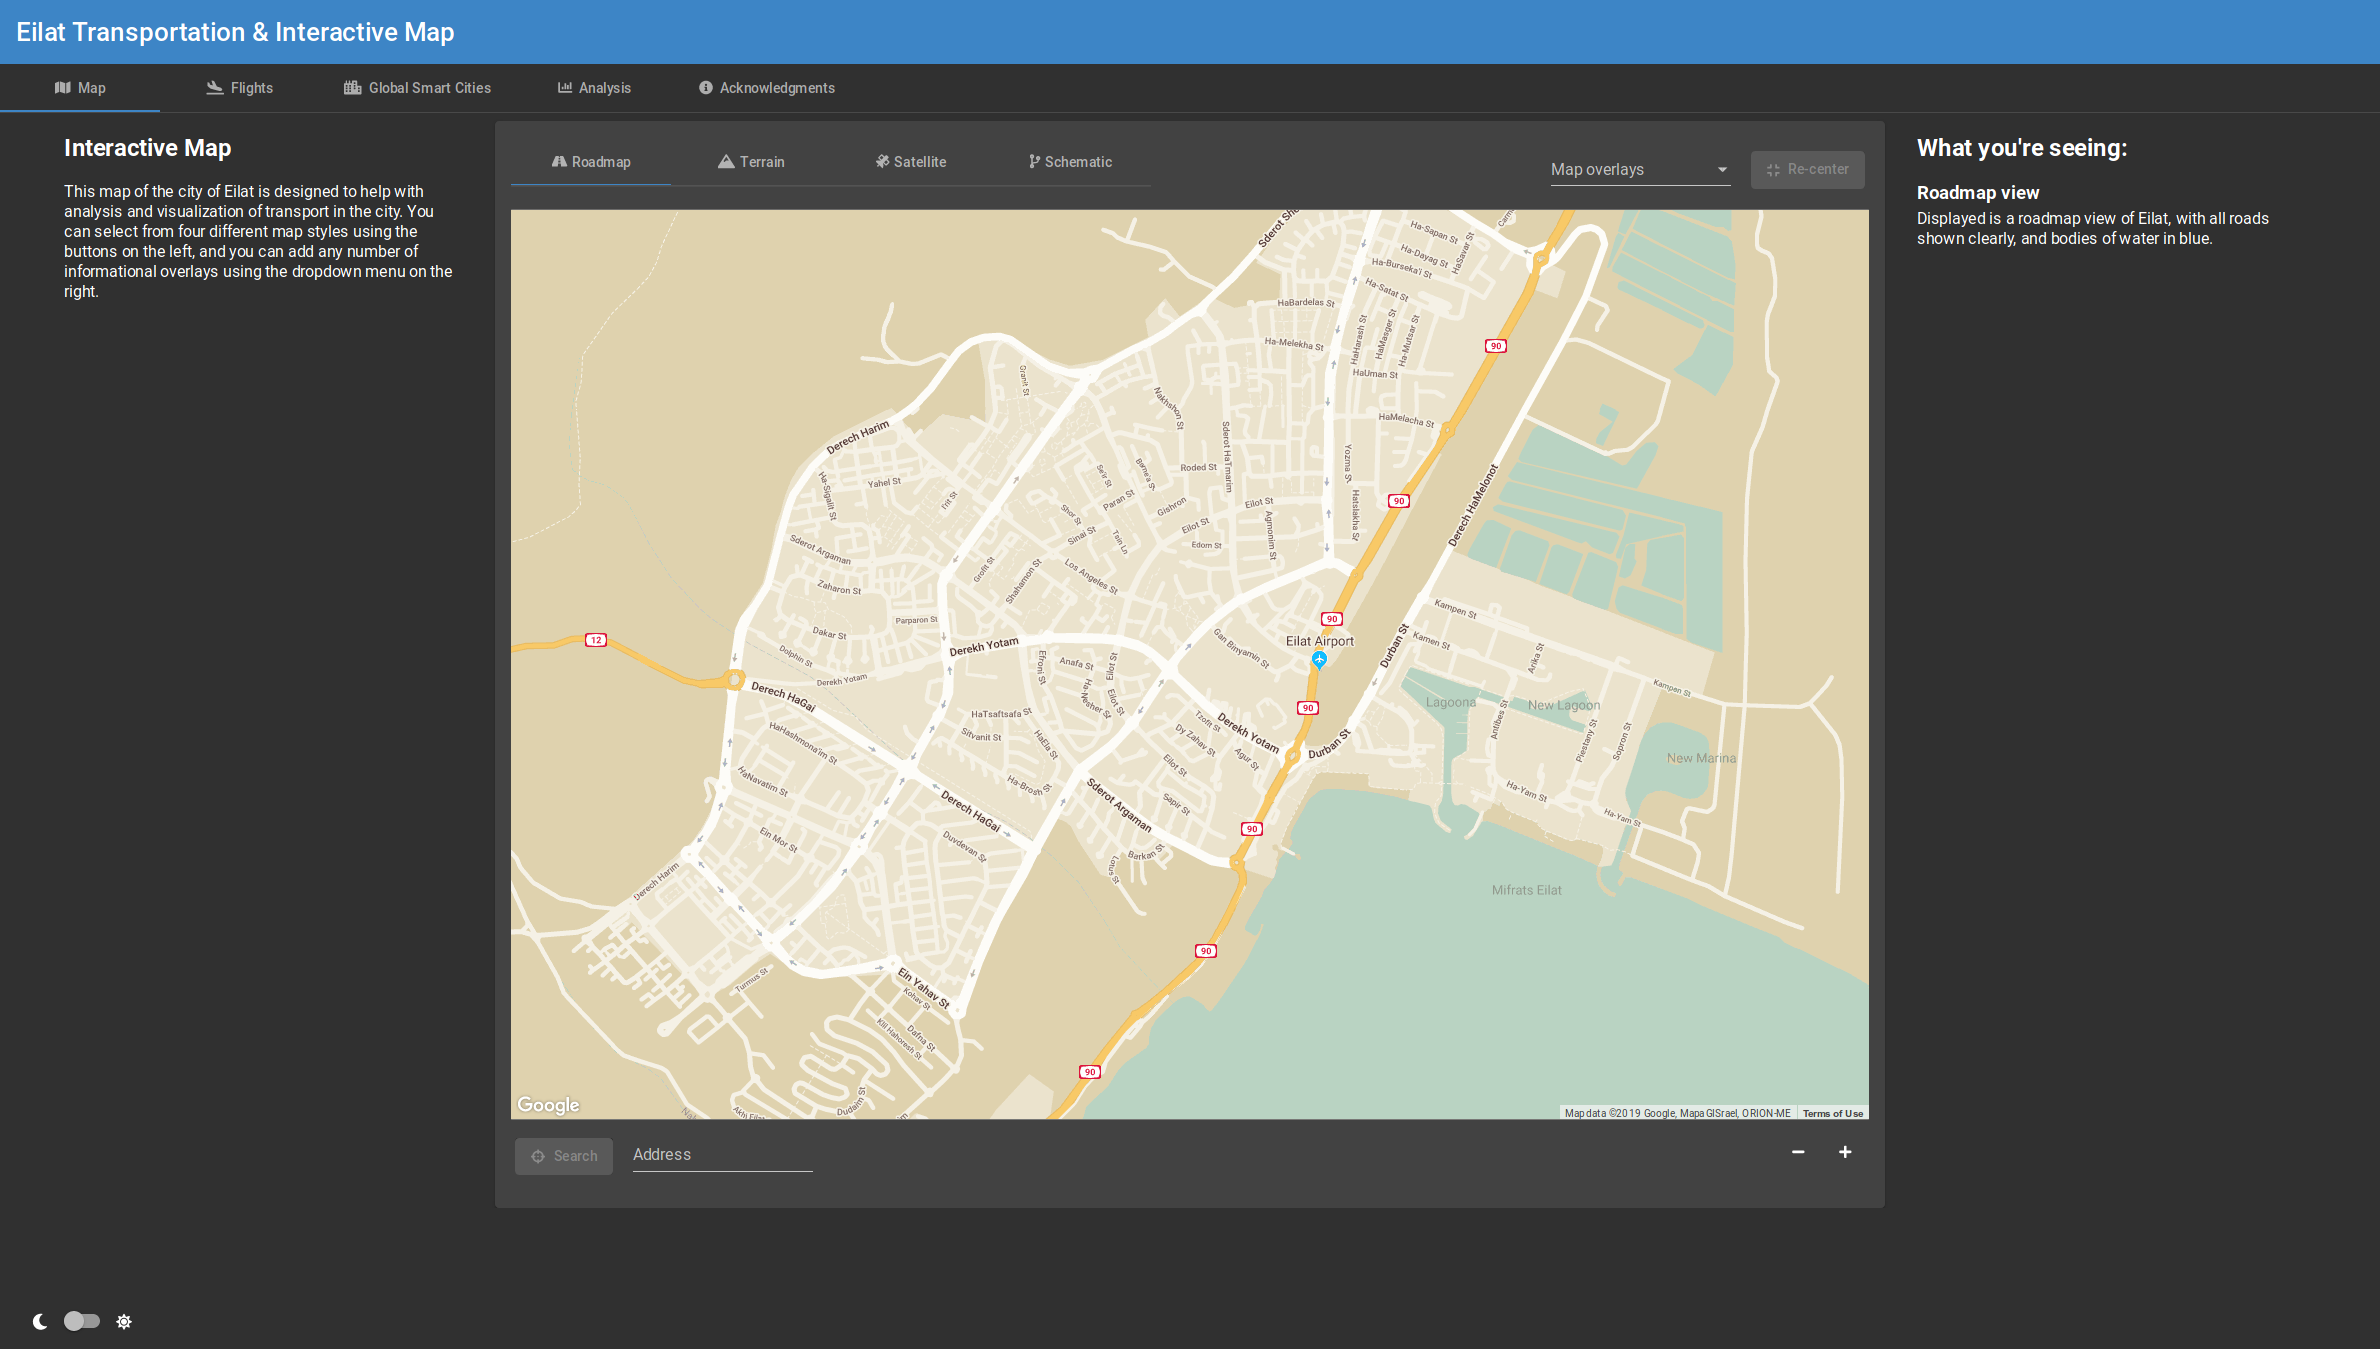
\includegraphics[width=1\textwidth]{images/site_map.png}
    \caption{Website default map view}
    \label{img:site_map}
\end{figure}

Figure \ref{img:site_map} shows the website when it first loads and the default map view, as generated by Google Maps. The left and right columns explain the purpose of the map and any features that might be visible. Four map view modes are available: traditional roadmap view, terrain view (for understanding the effect of topography on the city), satellite imagery view, and schematic view.

\begin{figure}[H]
    \centering
    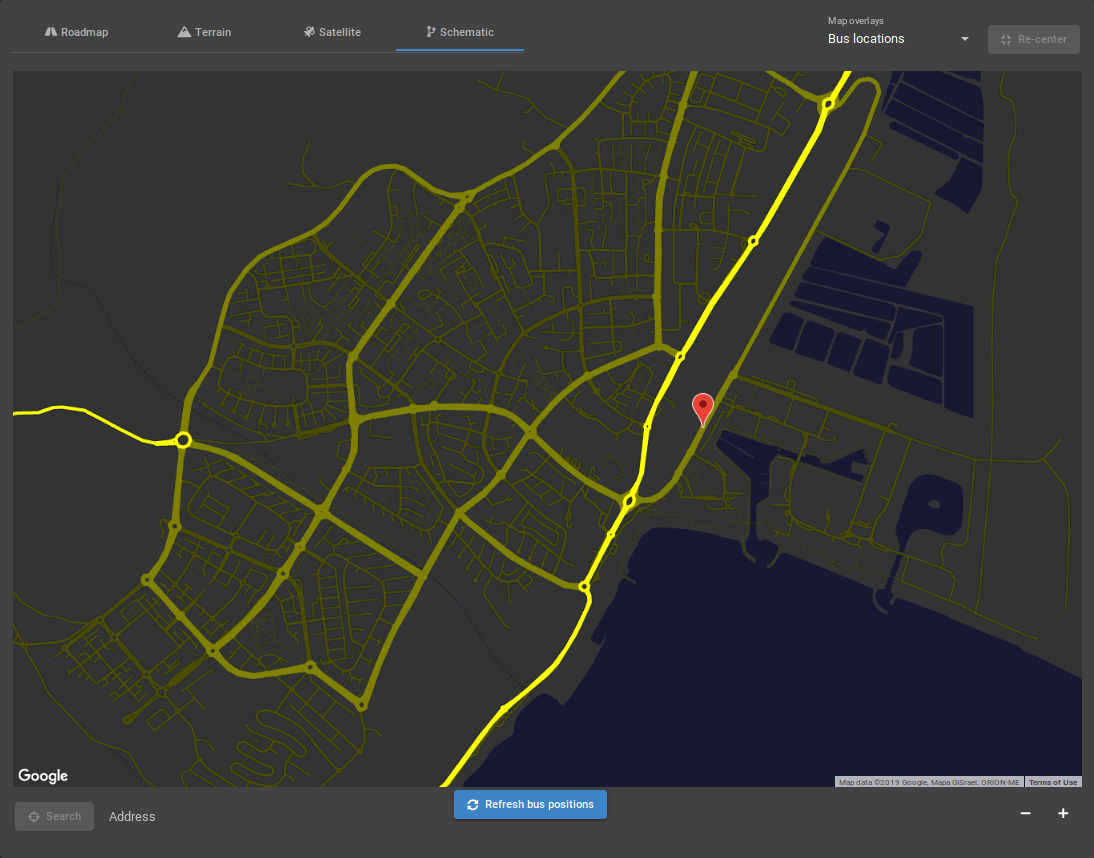
\includegraphics[width=1\textwidth]{images/site_map_schematic.png}
    \caption{Map schematic view with bus location markers} 
    \label{img:site_map_schematic}
\end{figure}

The "schematic view" in figure \ref{img:site_map_schematic} can be used to highlight road size using color; bright yellow lines indicate highways, darker lines are major cities arteries, and the darkest are for local roads. Any number of data overlays can be applied to a map type, such as bus location markers.

\begin{figure}[H]
    \centering
    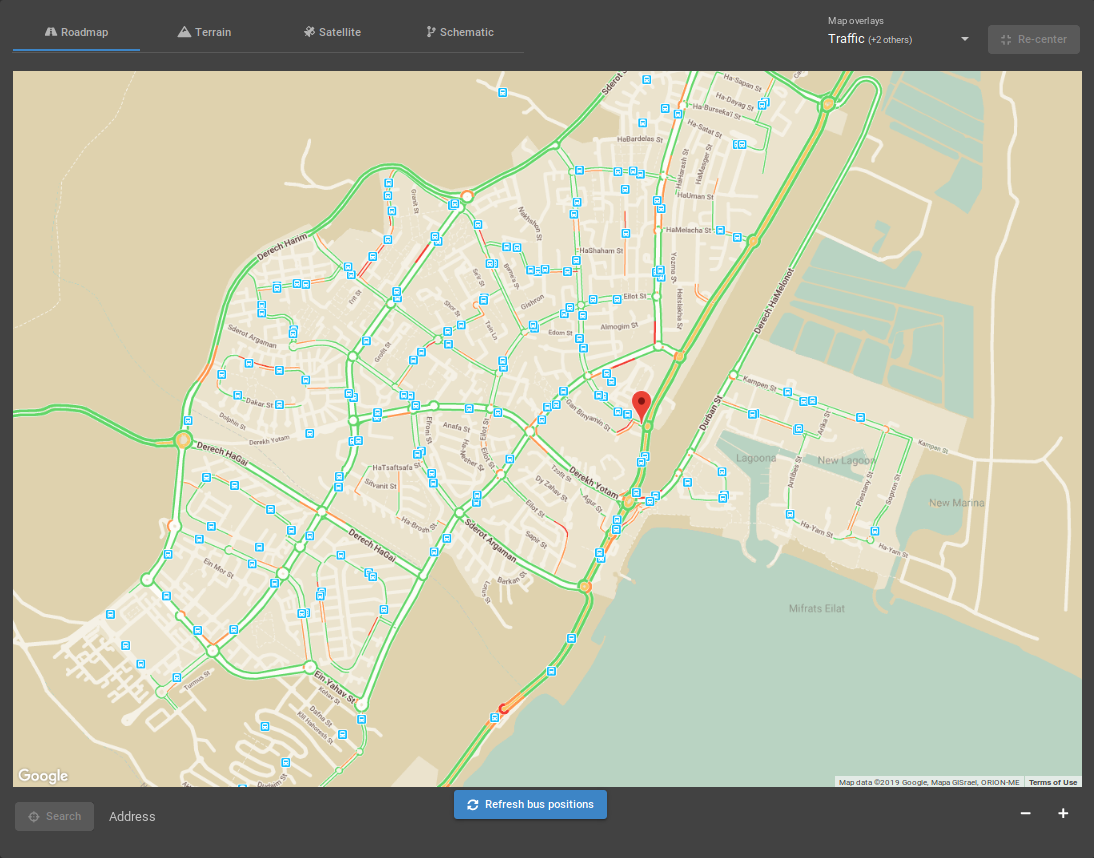
\includegraphics[width=1\textwidth]{images/site_map_traffic.png}
    \caption{Map view with traffic and bus location markers}
    \label{img:site_map_traffic}
\end{figure}

The view in figure \ref{img:site_map_traffic} shows live traffic data alongside locations of buses within the city (\textit{note: this image was taken on a Friday night as services in Israel begin to shut down, so there is only one bus in the city}), which can aid city planners both in understanding where traffic hotspots lie and in understanding how buses interact with traffic. Typically there are 10-12 buses in the city at any given time, many of them clustered together or spending long periods in areas of heavy traffic.

\begin{figure}[H]
    \centering
    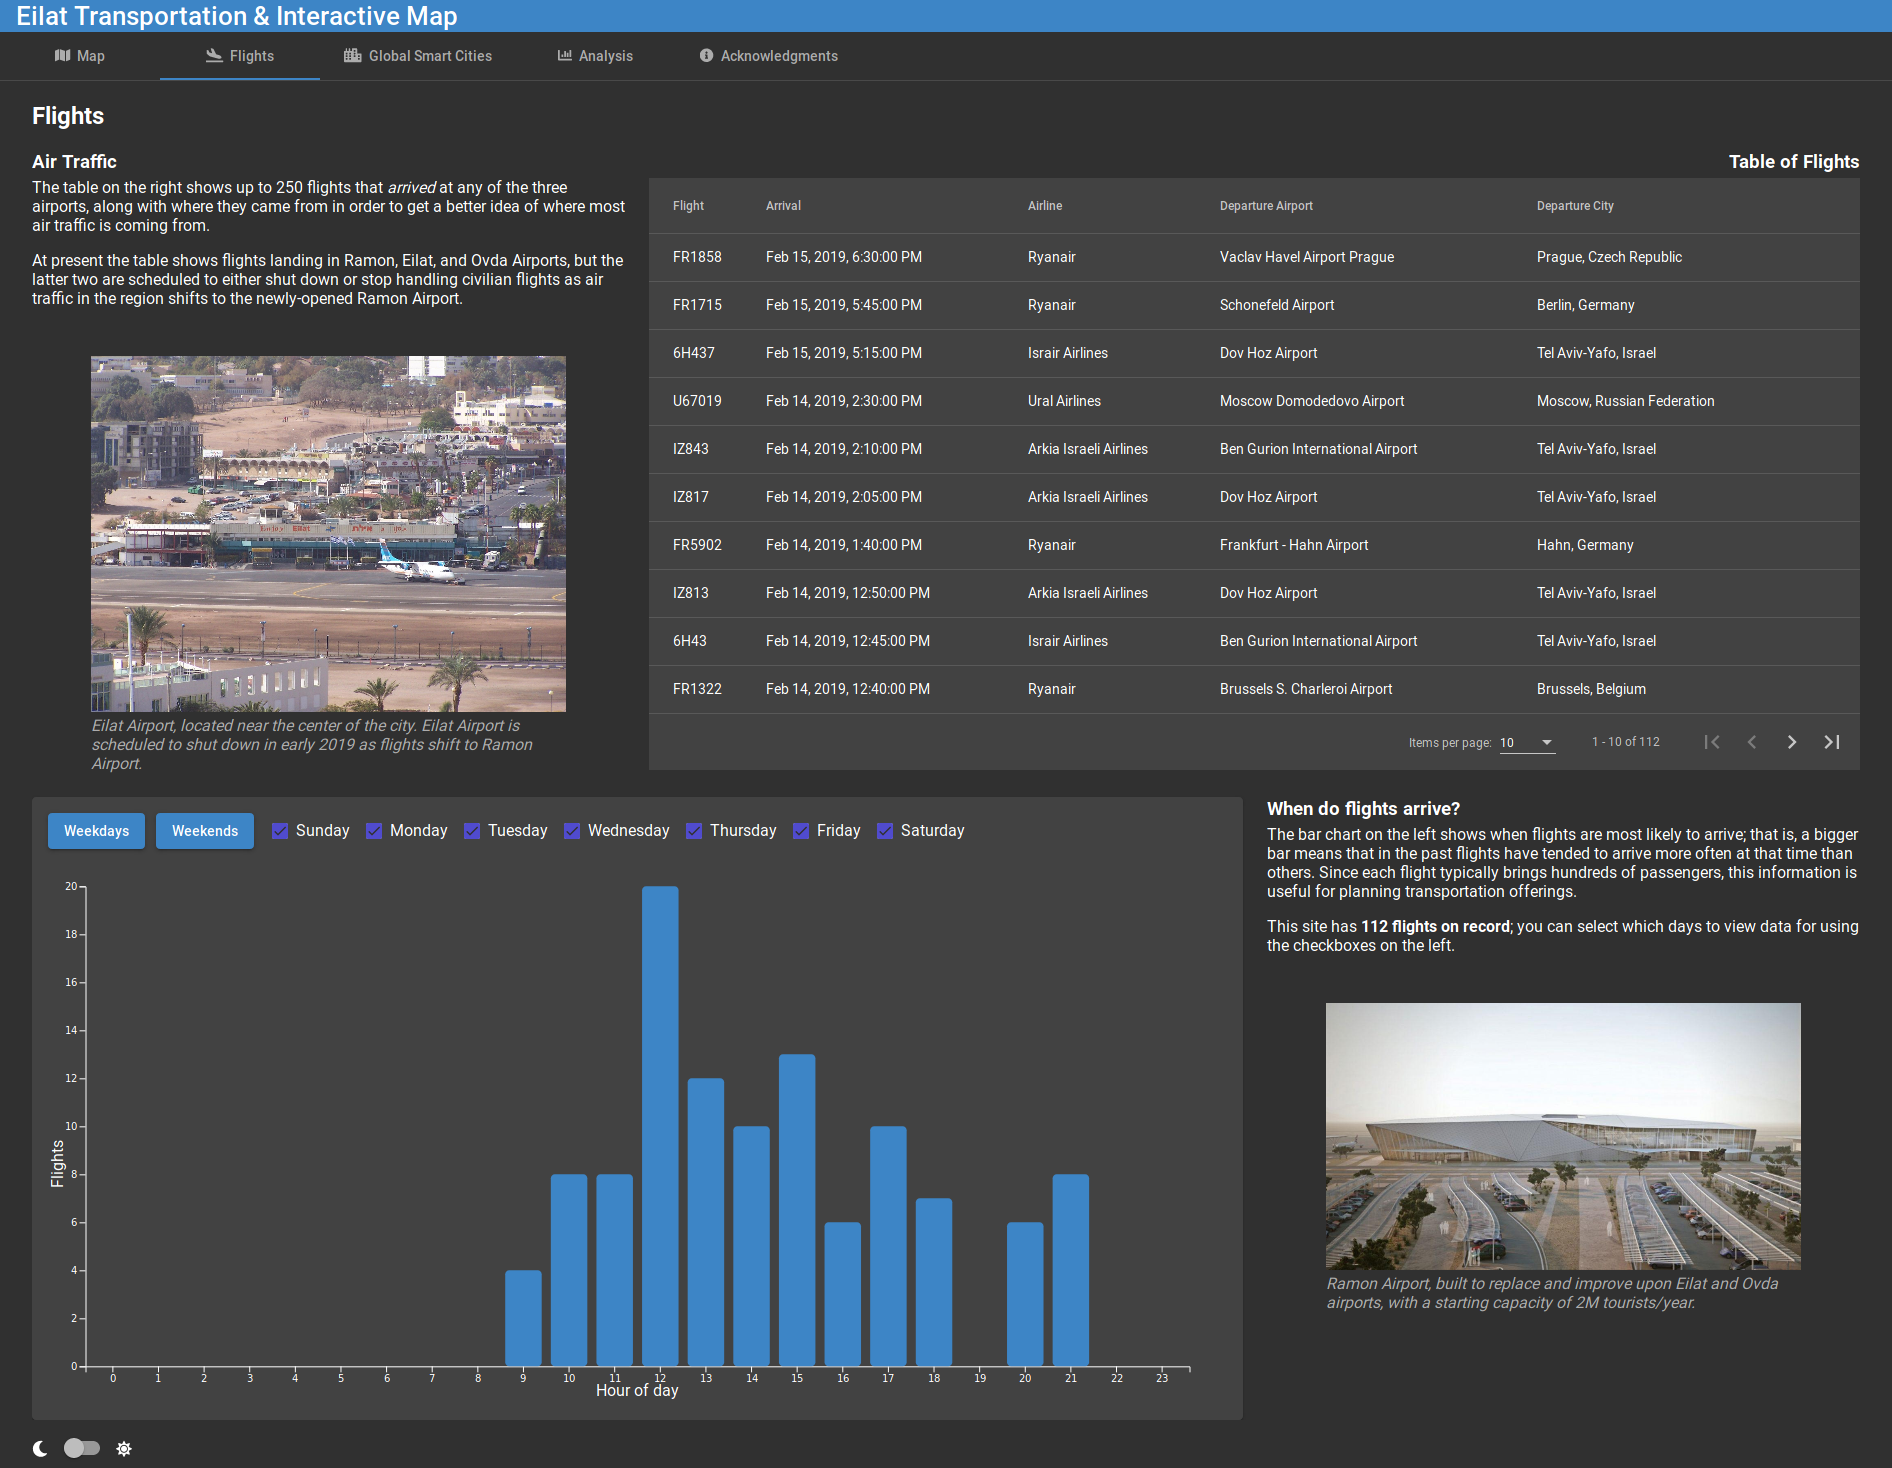
\includegraphics[width=1\textwidth]{images/site_flights.png}
    \caption{Website flights page}
    \label{img:site_flights}
\end{figure}

Figure \ref{img:site_flights} shows the flight data page, built using data on when flights arrive in Ramon, Eilat, and Ovda airports, despite that the latter two are scheduled to effectively shut down as Ramon takes over for air traffic in the region. The chart on the the top right shows a table of the last 250 flights into the region (useful to understand where tourists are coming from), while the histogram on the bottom left (figure \ref{img:site_flights_histogram}) shows flight arrival times. The table can be sorted by any of its headers, allowing users to quickly search for arrival times, airlines, departure locations, and so on.

\newpage
\begin{figure}[H]
    \centering
    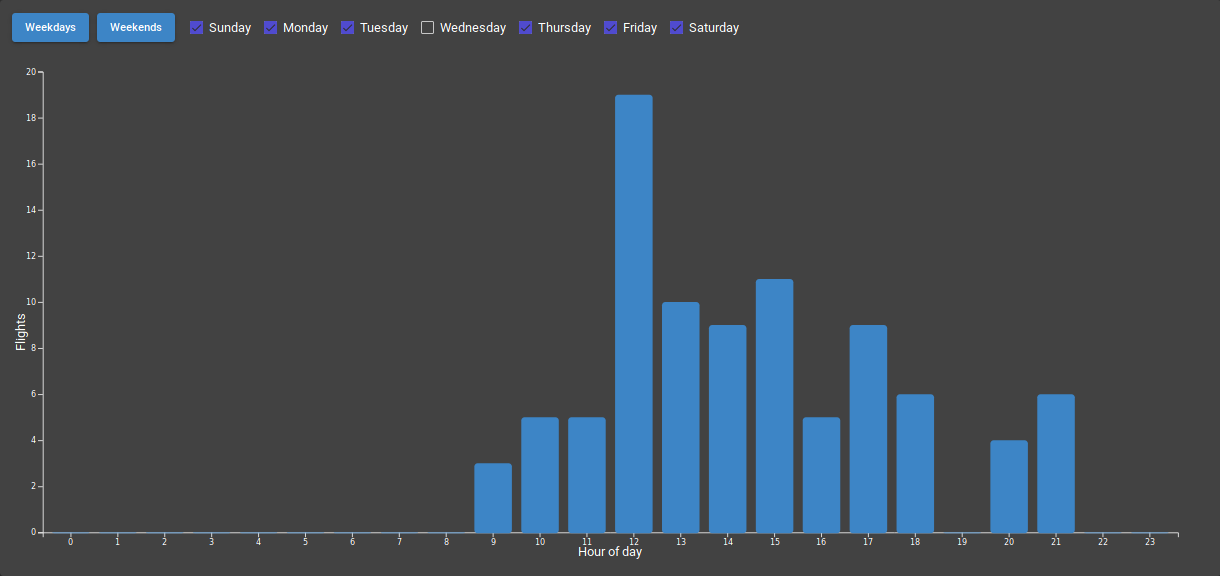
\includegraphics[width=1\textwidth]{images/site_flights_graph.png}
    \caption{Flight arrivals histogram}
    \label{img:site_flights_histogram}
\end{figure}

The histogram is a fully interactive chart designed to show when flights are most likely to arrive. The higher the bar on the chart, the more flights that have landed in the Eilat region at that time in the past, and thus the more likely it is that flights will land at that time in the future. Since airport traffic may vary by days, checkboxes can be used to select display of data for only certain days of the week. These can easily be toggled in groups using the "weekdays" and "weekends" buttons, which are included since air traffic on weekends is different than air traffic on weekdays.

% This part *probably* isn't needed, but what the hell. Someone feel free to delete it if you want.
\begin{figure}[H]
    \centering
    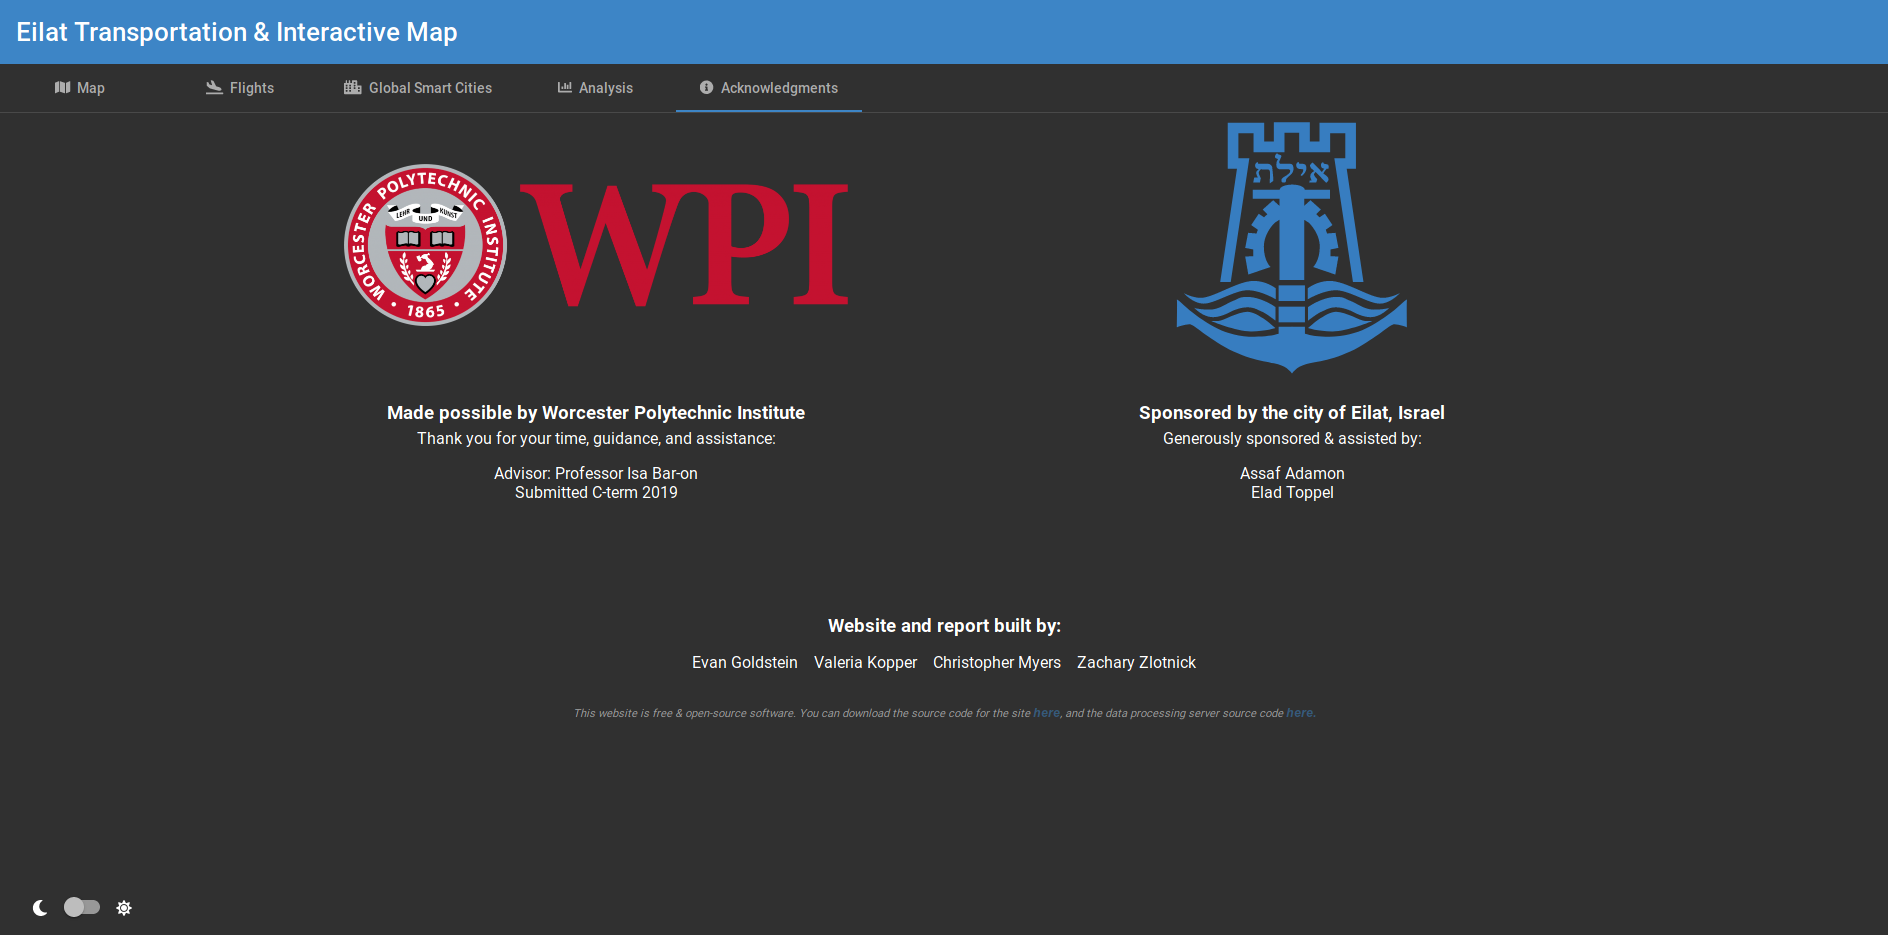
\includegraphics[width=1\linewidth]{images/site_about.png}
    \caption{Website acknowledgments page}
    \label{img:site_about}
\end{figure}

Finally, figure \ref{img:site_about} shows the site's acknowledgments page, which thanks WPI and our sponsors for their time and assistance.

\subsection{Implementation Details}[Christopher M.]
The website is structured into two components: the front-end website itself (shown in the website overview section), and the data server responsible for processing data and sending it to users of the site for display. The source code for the site is freely available \href{https://github.com/c7c8/Eilat-Transport-Map-Site}{here} and the server code is freely available \href{https://github.com/c7c8/Eilat-Transport-Map-Server}{here}. Both are designed to operate reasonably independently from each other: the site can receive data from any source, and the data server will provide data to any application.

\subsubsection{Website}[Christopher M.]
The website is built using the Angular 7 framework to manage data, user interaction, and render the site. Each page is built as its own module, operating independently from the others, making the site much easier to understand and expand, should a future IQP continue development of it. The website uses Angular Material, a library of user interface elements and styles aimed at implementing Google's "Material" design language \cite{Google2019}. As a result the site is easy to use, accessible, touchscreen-friendly, and incorporates design elements and behaviors that should be familiar to most users.

The mapping portion of the website is built on top of the Google Maps API, provided as part of the Google Cloud Platform. The API allows display and styling of maps as provided by Google, geocoding addresses to coordinates (this is how the map "search" feature is implemented), and more beyond simple maps of the city. In particular the service allows for the display of overlays and arbitrary datapoints; this is how the traffic overlay is implemented, or how the map is able to display markers to indicate the location of buses within the city. Unfortunately this service is not without cost. The map is unable to display \textit{historical} traffic data as Google simply does not supply it, and requires an API key (to access to the API) to function. API keys can be generated using the Google Cloud Platform console and will not incur any cost, but must be provided by the sponsor in the event they make a clone of the website. The website is also fully configurable and can be made to source data from any server. This makes it trivial for the sponsor to set up duplicates of the site as needed.

\subsubsection{Data server}[Evan G., Christopher M.] \label{sec:data_server}
The data server was written in Python 3 using the Flask server microframework, both chosen for rapid development, minimal up-front requirements, and light footprint. The server provides a small API to request data on three things: the most recent 250 flights landing near Eilat, a data analysis on when those flights land, and the locations of all buses within the city.

Flight data is provided by the \href{https://www.flightstats.com/v2/}{FlightStats API} from FlightGlobal, which allows a lookup of all flights arriving at an airport over a period of six hours in only one API request. Just as the Google Maps API requires a key, so does the FlightStats API, but in a more limited sense. This server has been built on top of a trial account that limits the user to 1,000 requests per month, after which requests must be paid for. Consequently the server is set up to retrieve flight data once every 6 hours exactly, store it in a MySQL database for later analysis, and deliver to the website on demand. When the 1,000 trial requests run out, the server will no longer be able to retrieve new data with the same key but will still be able to serve cached data. Similar to the website, the server is also fully configurable and can be set to use any API key and MySQL database.

To analyze data on when flights land, flights are counted by hour and slotted appropriately into a 7x24 matrix (7 days per week, 24 hours per day). The data is then sent off to the site for display on the histogram.

The data server retrieves public transportation information from two sources: the Service Interface for Real-time Information (SIRI) API (specifically the SIRI Stop Monitoring (SM) service) and General Transit Feed Specification (GTFS); both are provided by Israel's Ministry of Transportation. SIRI SM provides real-time information on bus stops, the estimated arrival times of buses at each stop during a given timeframe, and the current location of those buses. GTFS provides static information on public transportation, including bus stop information, scheduled stop times, and bus companies. The GTFS information is stored in the MySQL database and bus stops in Eilat are retrieved by filtering all bus stops in Israel by longitude and latitude. The ID numbers of the bus stops are fed into SIRI SM. From the SIRI response we get the location of all buses currently in Eilat.

\newpage
\section{Analysis}\label{sec:analysis}
\subsection{Website Data Analysis}
Data from the website provides useful information on how congestion, bus patterns, and air traffic interact to affect the city's transportation network.

\subsubsection{Congestion}[Christopher M.]
\begin{figure}[H]
    \centering
    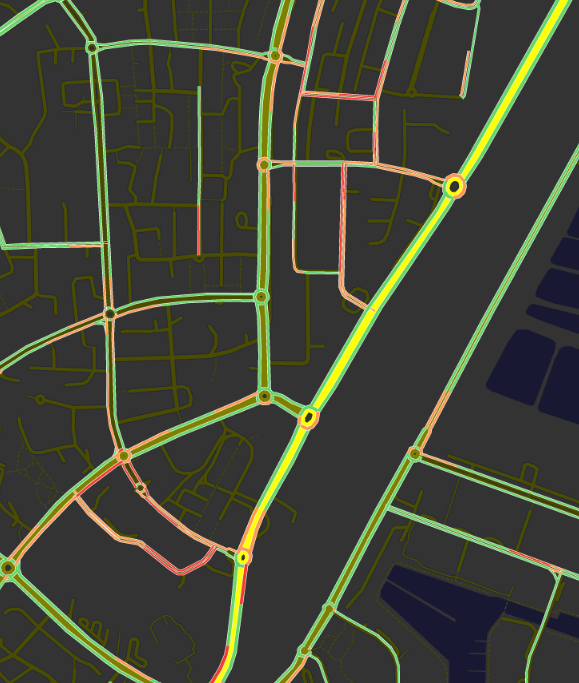
\includegraphics[width=0.5\textwidth]{images/congestion.png}
    \caption{Schematic view of congestion in central Eilat}
    \label{img:eilat_congestion}
\end{figure}

Eilat's congestion problem is relatively focused --- although there is general congestion across the city, there are a number of hot spots along major city roads and the small local roads that connect to them. For example, figure \ref{img:eilat_congestion} shows a schematic view of the region next to the airport with heavy congestion along the local roads stemming from it. This problem is particularly evident along route 90 (pictured) as traffic exits the route along the various traffic circles. While these traffic circles are good for low-medium traffic, they evidently result in more congestion and stop \& go traffic near their exits. Sometimes these traffic circles even result in drivers leaving route 90 at sub-optimal intersections. Ideally a road branching off a much larger or faster one should a large road, but according to the schematic view one of the most heavily congested roads (bottom left) is in fact a small local road.

\subsubsection{Bus patterns}[Christopher M.]
\begin{figure}[H]
    \centering
    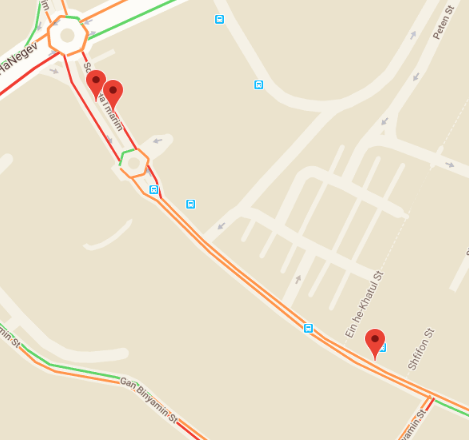
\includegraphics[width=0.6\textwidth]{images/bus_clump_1.png}
    \caption{Groups of buses in high-traffic zones near central Eilat}
    \label{img:bus_clump_1}
\end{figure}

Live bus data from the map reveals that buses in Eilat are vulnerable to spending time in highly congested roads near the city center like the one in figure \ref{img:bus_clump_1}, significantly slowing down the route. Many bus routes travel through these high-traffic zones in the tourist-oriented parts of the city, even along smaller local roads like the one in the figure.

Buses have also been observed grouping together into one area in these high traffic zones. Good public transport should ideally be distributed throughout the city, but frequently these buses can be found in groups of 3-5 near or along highly congested roads in the center of the city. Figure \ref{img:bus_clump_1} shows 3 buses within a space of 200 meters, with more in the same general area (not shown) in the city.

\subsubsection{Bus Stops}[Evan G.]
Bus stops are highly concentrated in residential areas and frequently in close proximity to one another (often as close as 50 meters). For most neighborhoods, a walking distance of no more than five minutes from home to the bus can be achieved by only one or two bus stops.

City-wide, there is almost always at least one bus stop within a 5 minute walking distance. The radial routes covering outlying areas run every 60 minutes, and a choice must be made between a longer wait and a longer walk. Additionally, the bus ride itself often takes longer than walking along the most direct route. In the city center, stops are closely spaced and accessible, but the southern coastline along route 90 (e.g. Mosh beach and Coral Reef) is not accessible by bus at all.

\subsubsection{Flights}[Christopher M.]
\begin{figure}[H]
    \centering
    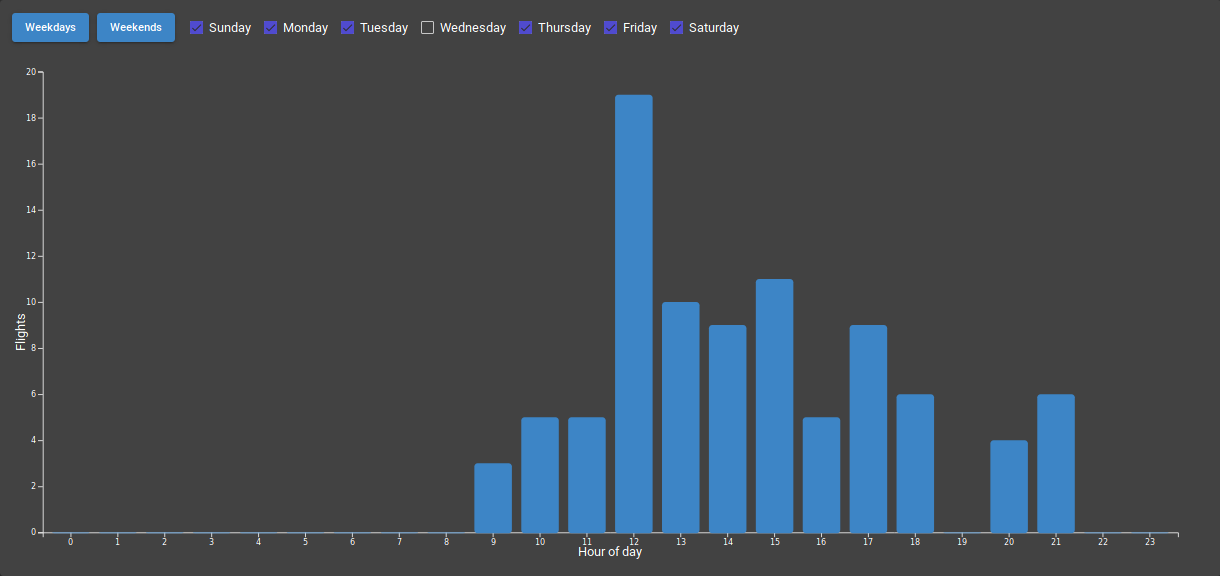
\includegraphics[width=1\textwidth]{images/site_flights_graph.png}
    \repeatcaption{img:site_flights_histogram}{Flight arrivals histogram}
\end{figure}

According to flight arrival information in figure \ref{img:site_flights_histogram}, most flights arriving in the Eilat region land between 9:00 and 21:00 (a 12 hour span). Flights in the morning are less common than flights in the evening, and there is overall only a minor decline in flights over the course of the evening. Accordingly, any airport shuttle service should be more focused on the evenings than the mornings, and nighttime service should be a low priority.

It is important to note that this data is currently flawed: data collection is run every 6 hours (see \S\ref{sec:data_server}), but when the data for \textit{this} graph was collected, data collection was invoked manually by one of the site programmers. This means there was generally good coverage of daytime air traffic, but past 22:00 coverage of incoming flights was minimal to none, since site programmers were not active on the site to trigger data collection. This data collection process will be automated upon final site deployment to correct the problem and ensure city planners have access to better data.

\begin{figure}[H]
    \centering
    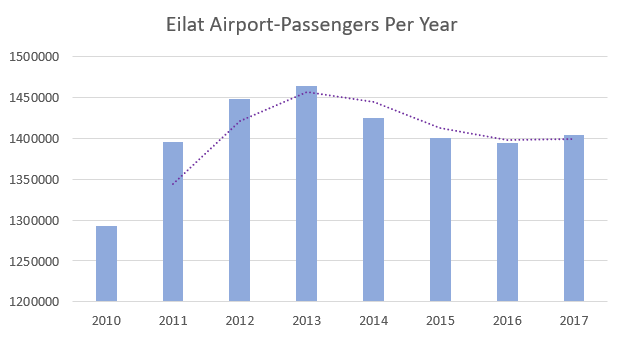
\includegraphics[width=0.75\textwidth]{images/passengers_per_year.png}
    \caption{Passengers per year arriving at the Eilat Airport}
    \label{img:passengers_per_year}
\end{figure}

\subsection{Tourist Traffic}[Evan G.]
According to data the Israeli Airport Authority 1.4 million passengers flew into Eilat in 2017. The number of passengers per month is estimated using the monthly tourism splits shown in figure \ref{img:passengers_per_year}.

\begin{figure}[H]
    \centering
    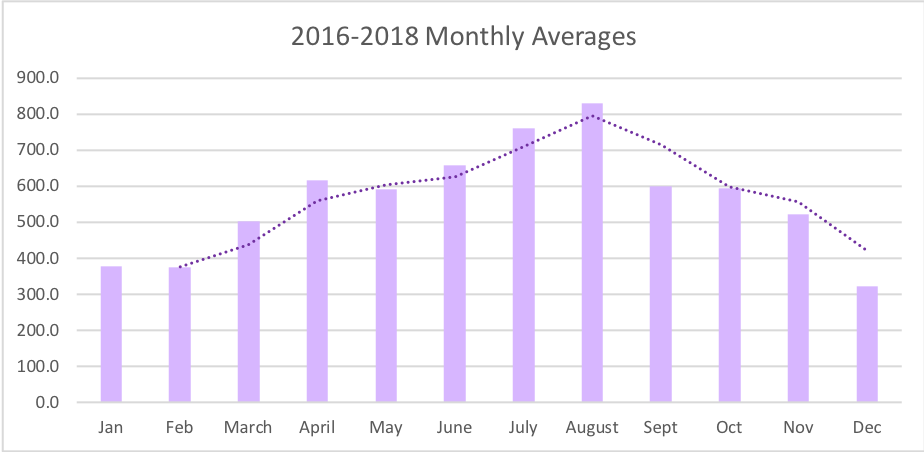
\includegraphics[width=.75\textwidth]{images/monthy_tourism_averages.png}
    \repeatcaption{img:monthly_tourism}{Monthly tourism}
\end{figure}

Eilat's tourists are mostly domestic, and typically drive or take the bus into the city rather than fly. In 2012 30\% of Israelis used buses \cite{Port2Port2012NewTransit,Petersburg2012LessTransit}; therefore, it can be estimated that 70\% of the 1.6 million tourists not arriving by plane in 2017 arrived by car. This equates to roughly 1.12 million tourists per year using cars in the city. Using monthly tourism splits (figure \ref{img:monthly_tourism}) from the same year and an average household size of 3.3 people \cite{CentralBuereauofStatistics2018IsraelNumbers}, the approximate number of tourist cars in the city per day for each month was calculated (shown in figure \ref{img:cars_per_day}). Eliminating these vehicles would result in a significant decrease in congestion.

\begin{figure}[H]
    \centering
    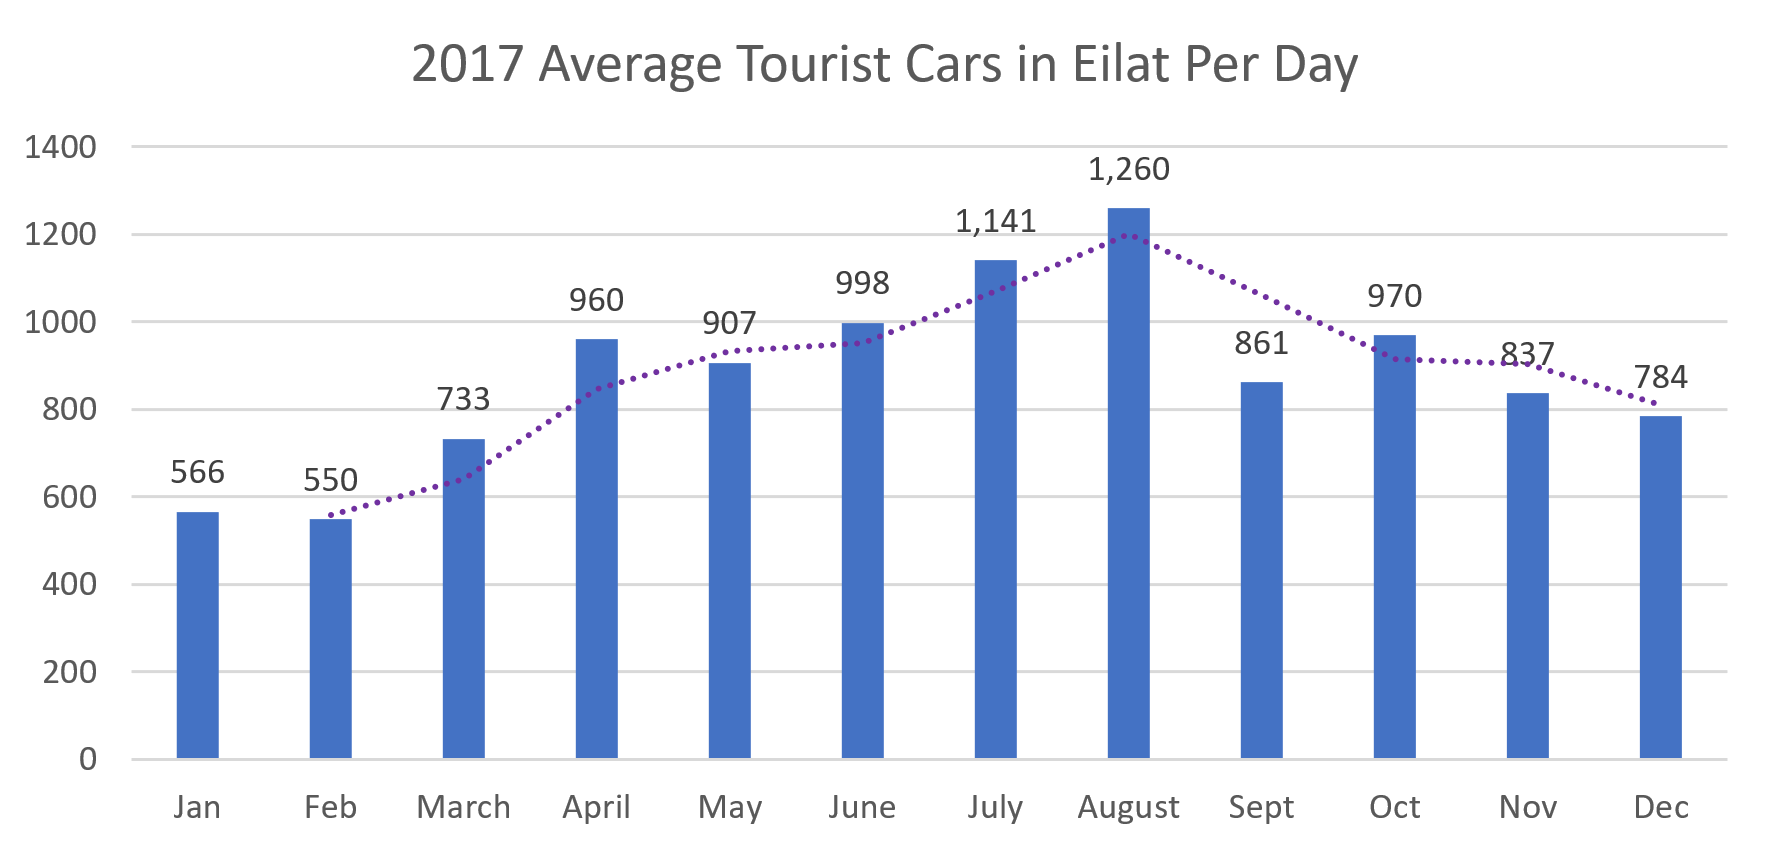
\includegraphics[width=0.75\textwidth]{images/cars_per_day.png}
    \caption{Average number of tourist cars in Eilat per day for each month}
    \label{img:cars_per_day}
\end{figure}

\newpage
\section{Suggested Improvements \& Goals}\label{sec:discussion}
\subsection{Addressing Congestion}[Valeria K.]
Eilat's major transportation problem of highly congested roads can be attributed to several factors: the inefficient bus system, high usage of private vehicles, and lack of alternative modes of transportation. Addressing them will be a major step towards improving Eilat's current situation, and each is detailed below, and the order of implementation is proposed and broken down into stages. (\S\ref{sec:implementation_stages}). In order to decrease congestion these all should be improved upon, which demands the creation of goals for Eilat to focus from now to 2040. Goals for Eilat should be based on the data gathered and analyzed regarding Eilat's current situation, the determined problems and influencing factors, as well as the models and goals proposed by case study cities. These goals should serve to identify the gap between Eilat's current situation and where it aims to be by 2040. Establishing the existing gap allows for the identification of the services needed to address each causing factor and goal in order to improve it. This can be majorly separated into three goals: improving transportation and its availability, decreasing private vehicle usage,  establishing mobility as a service. 

\subsection{Improve Public Transportation and Availability}[Valeria K.] \label{sec:disc_improve_transport}
The following goals can be established as tangible measurements of improving public transportation in Eilat and its availability by 2040. Be within 300-500 meters or within a 5-7 minute walk of a bus stop from any point within the city, established through the standard adopted by most case study cities; limit wait time at a bus stop to 10-15 minutes, determined by a logical standard on waiting time outside during extreme summer heat; decrease travel time, once on the bus, to 20 minutes from point A to point B (anywhere within the city), based on direct travel times by car; increase the percentage of population that uses public transportation, both residents and tourists, which is a standard measurement of improvement. 

In order to increase the percentage of the population (including tourists) that uses public transportation there is a need for investment and improvement of the bus system. Walking to a bus stop should take between 5 to 7 minutes from anywhere in the city. Existing bus routes should be reevaluated and changed to reflect traffic congestion and user demand. For more efficiency shorter routes that target specific areas in the city and that are repeated more frequently can be implemented. This can focus on adding more radial routes that target smaller areas, such as residential neighborhoods, and have fewer stops within each of them. This should maintain that walking to a bus stops should not take longer than approximately 5 minutes from anywhere within these neighborhoods, despite the fewer bus stops. In addition, designating more direct routes that cross the city, with more frequency and fewer stops. Some of these direct routes should be focused on bringing people from areas further away to the city center and other trip generators. Overall, bus routes need major restructuring to better serve the needs of the population and decrease travel and wait times. 

The implementation of shuttles in addition to the existing bus system is worth considering. There are large residential zones in the western part of the city. During peak times most people tend to commute towards the industrial zone and the hotel zone (due to most jobs being within these two areas). This accounts for presumably 59.9\% (population within standard working age) of the population commuting to similar locations during similar times. Given that private vehicles account 56.6\% of modes of transportation in Eilat it reasonable to deduct that this section of the population is greatly adding to congestion during these times.Adding a shuttle system that works during these times to target specific neighbors and take residents to their work area and back would help promote the use of public transportation. A similar alternative, if the shuttle system was not implemented, would be to create designated bus routes specifically for work commutes.
    
If public transportation is more efficient (meaning it takes less time to get from point A to point B) and it is more convenient (in that bus stops are close by and waiting times are shorter) more people are much more likely to use public transportation as the main form of transportation within the city. It is plausible that if more people use public transportation the use of private vehicles will decrease, which in turn will aid in alleviating congestion. Quicker bus rides and also be achieved by installing sensors throughout out the city can allow for smart traffic management. This would be mostly focused on major roads that suffer from the majority of the city's congestion, and would lead to smoother traffic flow. Introducing traffic lights that are phased based on traffic is what would permit this, and it would minimize the stops necessary when traveling from one side of the city to the other.

Providing a user friendly experience can also be greatly beneficial. This can be accomplished by having an app that allows for digital payment (minimizing interactions and the language barrier with bus drivers). The app can also include real time data provided through sensors in order for bus schedules to reflect update times, which serves to reduce wait times. It should also provide directions as to how to get to the nearest bus stop and directions to your final destination from the nearest bus stop. The app should be offered in languages additional to Hebrew in order to accommodate international tourists. 

\subsection{Decrease Private Vehicle Usage}[Christopher M.]
An obvious solution to reducing traffic is to reduce the number of cars in Eilat, or more specifically the number of private vehicles. Naturally this would lead to increased reliance on public transport and therefore fewer cars on the road, decreasing congestion and \textit{increasing} the effectiveness of public transport like buses. This will cause more people to use public transport and get off the road, and so on --- a feedback loop. The same is true in reverse, though (more traffic means ineffective public transport, meaning fewer people using it), so getting cars off the road and promoting public transport will require serious up-front effort and policies until traffic decreases enough.

There are a number of policy options available for getting cars off the road. The most immediate possibility is to provide direct incentives to residents to reduce the number of cars they own, like tax breaks for having one car or less per household, tax write-offs for using public transport, or penalties for owning more than one car. Since Eilat is a city and can't affect state-level taxes, implementation of excise taxes on cars in the city may be the best option; it depends on what Israel's tax laws look like.

Another possibility to remove cars from the road is carpooling. To make carpooling more attractive, lanes could be marked as allowing only vehicles with more than a set number of people in their car. A further option is to require payment for parking (ex. parking meters) in a progressive fashion that increases as you approach the city center or other designated zones. This would discourage people from driving through high-traffic zones to their final destination. Discounts could also be applied to those who choose to carpool, further helping to remove cars from the road. For more policy examples, see \S\ref{sec:policies}.

As for policies aimed at Eilat's tourists, improved public transportation is likely the best overall solution, depending on how tourists tend to get into the city. Those who fly or take buses into the city are more suggestible to using other transport than those who drive, so policies should be aimed at the two groups independently. Someone who didn't drive to Eilat should be made readily able to explore the city without renting a car or calling a taxi, meaning fast and cheap transport from Eilat's hotels is a must. On the other hand, someone \textit{with} their own car must be incentivized to leave it behind, and won't be affected by tax breaks or penalties like an Eilat resident would. Affordable parking outside main areas of the city (already planned or in effect, see \S\ref{sec:parking}) combined with effective public transport is likely the best passive way to convince them to leave their cars behind. For a more active or penalty-based solution, the parking meter solution from earlier would similarly affect tourists, but at risk of dissuading them from staying in the city too long or exploring local businesses (nobody likes frequently paying for parking).

Care should be taken to ensure that making driving \textit{un}attractive comes after making pedestrian travel itself attractive. Eilat is situated in a desert and frequently reaches over 45\textdegree{} C during the summer --- peak tourism season. Residents and tourists alike should be made to feel comfortable walking, both by providing shade from the sun along major thoroughfares and by ensuring that pedestrian travel is never longer than absolutely necessary (i.e. dense public transport).

\subsection{Establish Mobility as a Service}[Zachary Z.]    
It is important to note that the previously mentioned reduction in private vehicle usage should result in an uptick in the use of provided mobility services. The definition of an effective service can vary based on the associated price, convenience, reliability, weather, safety, or travel time. In order to detach citizens in Eilat from their steering wheel, services across the board will need to focus on addressing the gaps existing services exhibit in accordance to these factors. 

The variance in demographics will make the selection of services that reflect the individualized needs of cities significantly more difficult in comparison to other popular destinations. For example, cities like London, Bankok, and Paris were the three most popular tourist destinations of 2018; however, if you look at the tourist per capita ratio (tourists to residents), only Paris exceeded Eilat. Both London and Bankok were well under 3 compared to Eilat's ratio of 5, with Paris being about 9 \cite{Murray2018MostInsider}. This means that, especially at times of peak tourism during the summer, the services need to reorient themselves toward the average tourist: typically someone with less than average knowledge of the existing system, who is willing to spend a reasonable amount, and may not speak Hebrew. Taking this into account, effective services for tourists will need to provide ease-of-use before anything else. In contrast, one of Eilat's 50,000 residents would likely prefer to see minimized travel times in junction with a minimized price. 

Ensuring accessible and affordable transportation are two goals for the services which should embody the consumer values above. In order to gauge the accessibility, the city can measure via surveys or tests the viability of getting from one point to another only 10 minutes slower than if they used their own private vehicle. This time should be measured from parking spot A to parking spot B for private vehicles, and will vary during times of peak congestion and/or peak tourism seasons. This goal would primarily interest Eilat residents the most, since they struggle morning and afternoon getting to and from work. For tourists, accessibility should be provided through an app interface which specifically targets the language and payment barriers. This includes providing routing information with associated stops and linked wayfinding apps for the "last mile."

Affordable transportation should be fairly similar for both parties. Currently, bus prices within Israel are extremely reasonable which is one of the largest advantages over other methods of transportation within Eilat. Taxi services are at a predetermined variable cost, in that riders are informed that their rides will be contingent on the traffic at the time and the distance. Keeping customers informed ahead of time what these costs are, similar to Uber and Lyft, would likely garner more users and be more desirable for tourists familiar with those services. This is entirely realistic given that taxi drivers often make up fares on the spot when riders fail to use the Gett app, and riders would feel less taken advantage of.

\subsection{Sustainability Considerations}[Valeria K.]
The city of Eilat has established it aims to be as sustainable as possible and there are multiple initiatives that can be implemented to achieve this. Overall, smart city technologies largely encourage environmentally-friendly considerations; therefore, any steps taken towards transitioning into a smart city will also further the city's sustainability initiative. Installed sensors can be used for sustainable purposes such as street light controls and management of public water usage (such as in parks; further descriptions of these technologies can be found in \S\ref{sec:smart_city_sensors}). Cameras can also be used to monitor the city's cleanliness, which could potentially be used to impose a littering fee. 

It is important to take into account the repercussions attached to adding certain technologies such as the energy consumption of sensors and traffic lights. A way to address this is to focus some of Eilat's efforts on renewable energy sources, especially solar energy due to Eilat's vast potential.

\subsubsection{EV Implementation}[Valeria K.]
Overall encouraging the adoption of EVs in Eilat can have many sustainability benefits. This would require the installation of EV charging stations throughout the city. Focusing EV efforts on public transportation, such as converting conventional buses to electric buses, can lead to greater benefits. This would allow for more buses to be added to the bus system without major environmental repercussions. Aiming to decrease private vehicles on the roads means that this should not be the main focus of EV incentives; however, getting the remaining cars on the road to be EVs would still clearly be beneficial to Eilat and should not be disregarded. 

\subsection{Implementation Stages}[Valeria K.] \label{sec:implementation_stages}
The city of Eilat can plan for changes from now until 2040 by dividing the transition into a smart city into four stages. These are described below and aim to serve as a guide that will address the aforementioned goals by decreasing congestion and improving the overall quality of life. See Appendix \ref{img:stages_graphic} for a visual representation.

\subsubsection{Stage 1: Setting the Stage}[Valeria K.]
Eilat should invest in the infrastructure necessary for the proposed improvements firstly by installing sensors and cameras throughout the city. City-wide WiFi should be improved, and this could be accomplished by establishing a partnership with cell carriers. The implementation of traffic lights in key congestion points should be evaluated, mainly because this would allow for future smart traffic management. 

Establishing uniform, efficient data collection is crucial for data analysis. Additionally, this allows for measurement of progress and comparison in the future. Crucial points of data collection would be: public transportation usage, available parking, traffic speed, and traffic density. This is a necessary starting point of data collection that by no means imply it should be limited to these aspects. Furthermore, an open data platform should be created. This allows for transparency and trust from citizens as well as collaboration from third parties. 

A program that will promote car-pooling should be developed. The city should also make an attempt of partnering with Waze through their Connected Citizens Program. If not, an equivalent for traffic data exchange should be explored.

Piloting heat solutions to address Eilat's extreme heat during the summer months is also important since it will help promote walk, biking, using electric scooters, etc. This can take the form of additional shade throughout the city, especially in zones that aim to prioritize pedestrians. 

An effective, user-friendly (for residents, domestic tourists and international tourist) public transportation app would be greatly beneficial. This can take the form of either improving the existing Moovit app or developing a new app. A main focus, at this stage, should be decreasing the language barrier between the user and the information, as well as human interaction (such as with bus drivers that solely speak Hebrew).

\subsubsection{Stage 2: Piloting Improvements}[Valeria K.]
Improving the existing bus system, given that it is the main form of public transportation, should be greatly emphasized. A bus system reform period should be established, which can later diminish and focus on continuous improvement. Adding more bus stops, especially in key locations, will lead to shorter commutes to bus stops. Optimizing bus routes is also important since they are currently inefficient and cover wide areas of that city that result in long waits and long travel times. Creating shorter routes that are more frequently repeated and target specific city areas would diminish both of these times. 

Programs such as car-sharing, bike-sharing and e-scooters should be established. Piloting the shuttle system, described in \S\ref{sec:disc_improve_transport}, should also occur during this stage. A defined time period for delivery services within highly congested areas can be set to times in which those streets are typically less congest. For example, from 14:00 to 16:00 in the city center. 

Further development of the transportation app should take place. Including digital payment would allow for minimizing unnecessary interactions, quicken boarding time. It would also allow for convenient seat reservation in advance. It could also be used to recharge the existing Rav Kav card payment system.

The sensor network should be expanded to include street light sensors and park water usage sensors, as described in \ref{sec:smart_city_sensors}, furthering sustainability initiatives dealing with energy and water conservation.

\subsubsection{Stage 3: Reinforcing the Existing System}[Valeria K.]
A parking restructuring should take place that would mainly restrict/reduce parking in the city center. In order to do so mass parking in the outskirts could be established. This would target domestic tourists driving into Eilat, and a shuttle could be provided to bring people to the city center. A tiered system should be implemented in which parking becomes more expensive the closer it is to the city center. Parking sensors should indicate where available spots are located, and an app should allow for digital payment (which will also serve to indicate the different pricing zones). Last minute mile options should be located near these parking lots.

Sustainability initiatives should include developing policies that encourage EVs. This can be further promoted by piloting EV taxis and buses. Road dieting should be implemented by designating lanes in roads to bikes. This should also be applied to car-pooling lanes. Additionally, the pedestrian center should be piloted in this stage.

The shuttle system can be fully deployed in this stage. It will focus on peak commute hours (that typically coincide with peak congestion times), and will work during a block during the mornings and afternoons. This should be complimented by setting set hours for drop-offs at schools, such as from 8:30 to 9:30.

\subsubsection{Stage 4: Enhancing the Experience}[Valeria K.]

A network feedback loop should be created in order to manage the frequency and the services offered. This should be sent to users through Waze, Google Maps, or an equivalent for them to have real time information that can allow them to reroute and plan to avoid congestion.

In this stage, sustainability stages should make EV charging stations widely available throughout the city, as well as have policies backing it up. Intra-city buses should be completely switched to EVs. The pedestrian center should be fully established. Vehicle access should be restricted through a tiered system based on data (how congested the area is) and proximity that allows for resident permits. Green spaces (possibly in the form of a public park) could be implemented to promote pedestrian use and improve quality of life. Options should be offered to within this central area, including walkways, bicycle lanes and shuttle services to and form. 

In this stage an integrated app would be incredibly beneficial by having all real-time data and services available in one place. This would encompass the previously mentioned public transportation data (including updating schedules and digital payment), directions up until the final destination (this can include directions to nearest bus stops), last minute mile options and access, and available parking (including digital payment).

%Apps should be developed to allow prepaying for public transit services, and should be available in multiple languages. Ideally, a single app would include options for buses, taxis/ride-sharing services, as well as last-mile solutions such as bikes and scooters.

% - Reorganized hours for certain services
% 	=> delivery/school/airport peak hours
% - Address the issues the bus ain't doing for the city rn

\section{Conclusion}[Christopher M.]\label{sec:conclusion}
The goals above are intended to guide Eilat over the next 20 years and are flexible, but there are some clear elements Eilat should strive for. Eilat needs to improve its public transport offerings to be more efficient, faster, and friendlier for the residents and tourists alike --- quality of offerings can be easily gauged by the percentage of the population using public transport. Offerings should be smartly managed and information should be both collected and delivered to users electronically. At a policy level the city should consider perks for going carless or carpooling, and penalties for those who drive in excess, but not impinge on quality of life and city accessibility. Finally, the city should be open to exploring pedestrian and mobility-as-a-service options to further reduce traffic and environmental impacts, while taking into consideration Eilat's climate and expansion plans.

% * Discuss the goals above and how to realistically measure them in the near future. Determine possible metrics for measure "good" prices, and "good" times.  
% Quality of life
% Prioritize pedestrians and cyclists

% Bibliography, automagically managed in APA style
\newpage
\doublespacing
\bibliographystyle{apacite}
\bibliography{refs}
\onehalfspacing
\newpage

\begin{appendices}
\section{Implementation Stages Graphic}[Valeria K.] \label{img:stages_graphic}
An infographic has been created to help visualize the smart city implementation stages and the recommendations presented on them, shown on the next page.

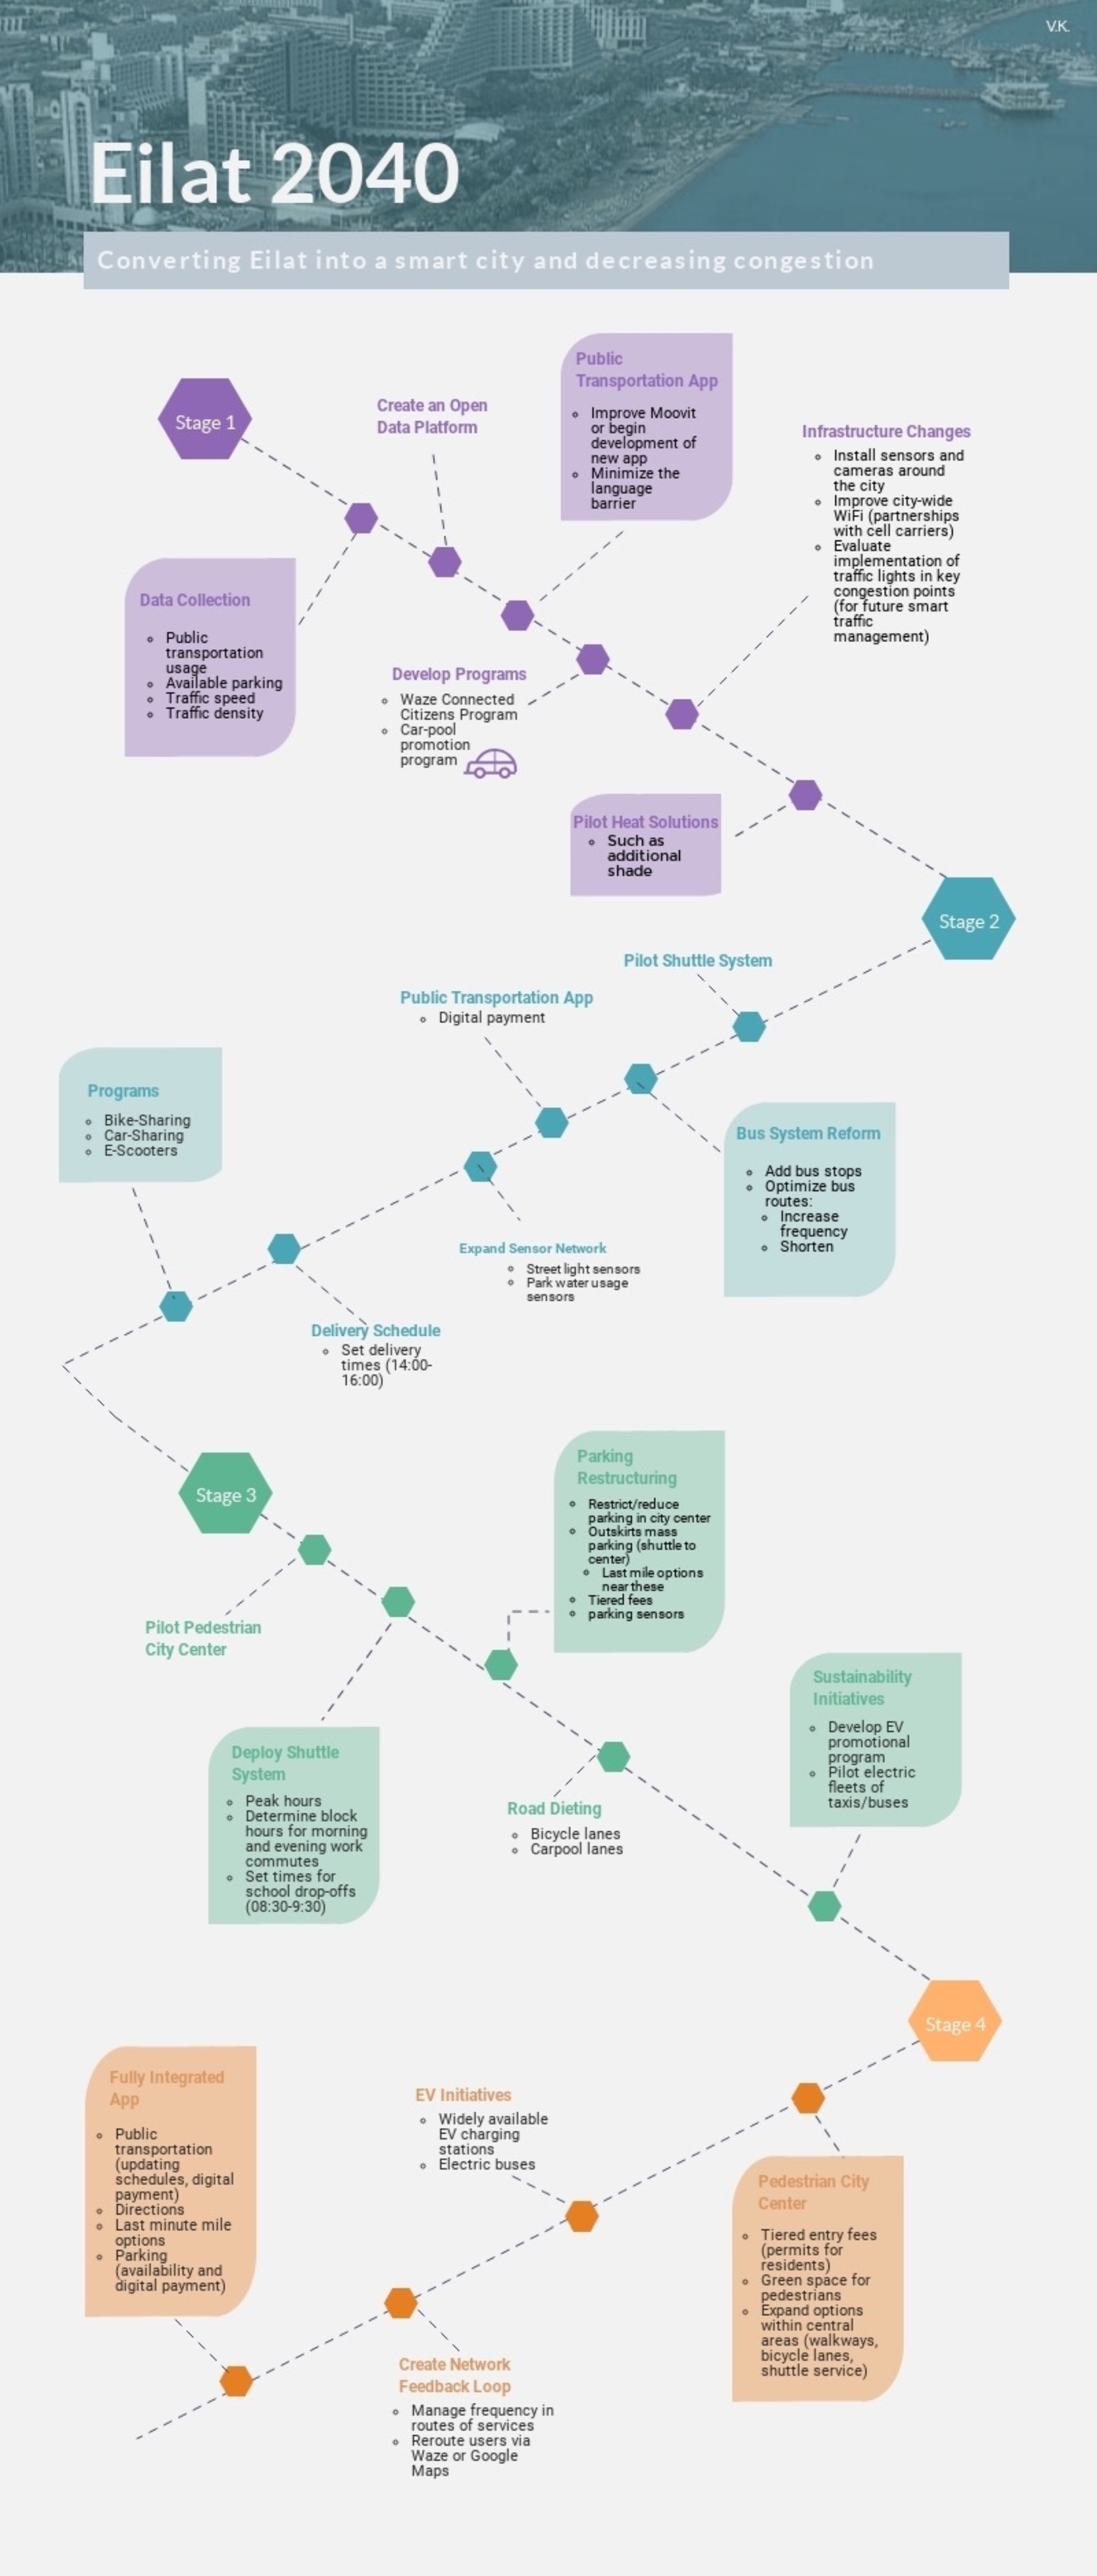
\includepdf{images/stages.pdf} 
\end{appendices}

\end{document}